\begin{comment}
\chapter{1. Числа, символы и фигуры}
\end{comment}
\newchapter{Числа, символы и фигуры}


\vrezka{<<Дети и наука>>: \href{https://childrenscience.ru/courses/sav/1/}{Урок 1. Числа, символы, фигуры}.

Конспект: Глава 1, разделы 1.1 Запись действий с отрезками, 1.2 Понятие натурального числа, 1.3 Визуальные доказательства. Глава 7, раздел 7.1 Построение рациональных чисел.}

\subsection*{Справочные сведения}

Операции сложения и умножения мы визуально ассоциируем со смещением по прямой вправо или влево. Вправо --- со знаком $+$, влево --- со знаком $-$. Смещение на несколько единиц вправо или влево --- это смещение на одноименное число шагов в данном направлении. В итоге операцию сложения или вычитания можно представить как путь по прямой дороге, который складывается из шагов, равных $+1$ или $-1$ в зависимости от направления.

Умножение задается с помощью прямоугольной сетки на плоскости. Имеем две координатные оси, на которых отложены, как и в одномерном случае, шаги-числа в обе стороны от точки $O$ с соответствующими знаками. Откладываем перемножаемые числа по обеим осям, получаем прямоугольник, состоящий из единичных квадратов. Число этих квдаратов, т.е. площадь прямоугольника, и есть значение произведения (см. рис. \ref{prod}).
\begin{figure}[hbt!]
\begin{center}
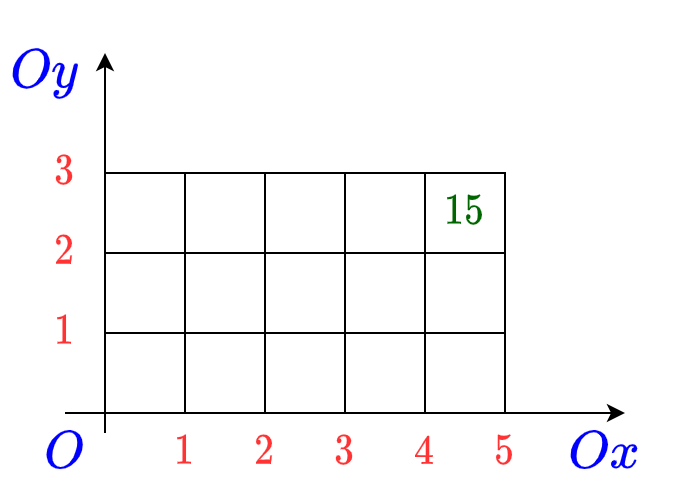
\includegraphics[scale=0.2]{../prod.png}
\end{center}
\caption{Произведение $5\cdot 3$.}\label{prod}
\end{figure}

В том случае, когда умножаются числа, оснащенные знаками, применяется правило ориентированной площади, т.е. знак выбирается в зависимости от направления оси наблюдателя, для которого порядок множителей всегда соответствует повороту против часовой стрелки (см. рис. \ref{mult}).
\begin{figure}[hbt!]
\begin{center}
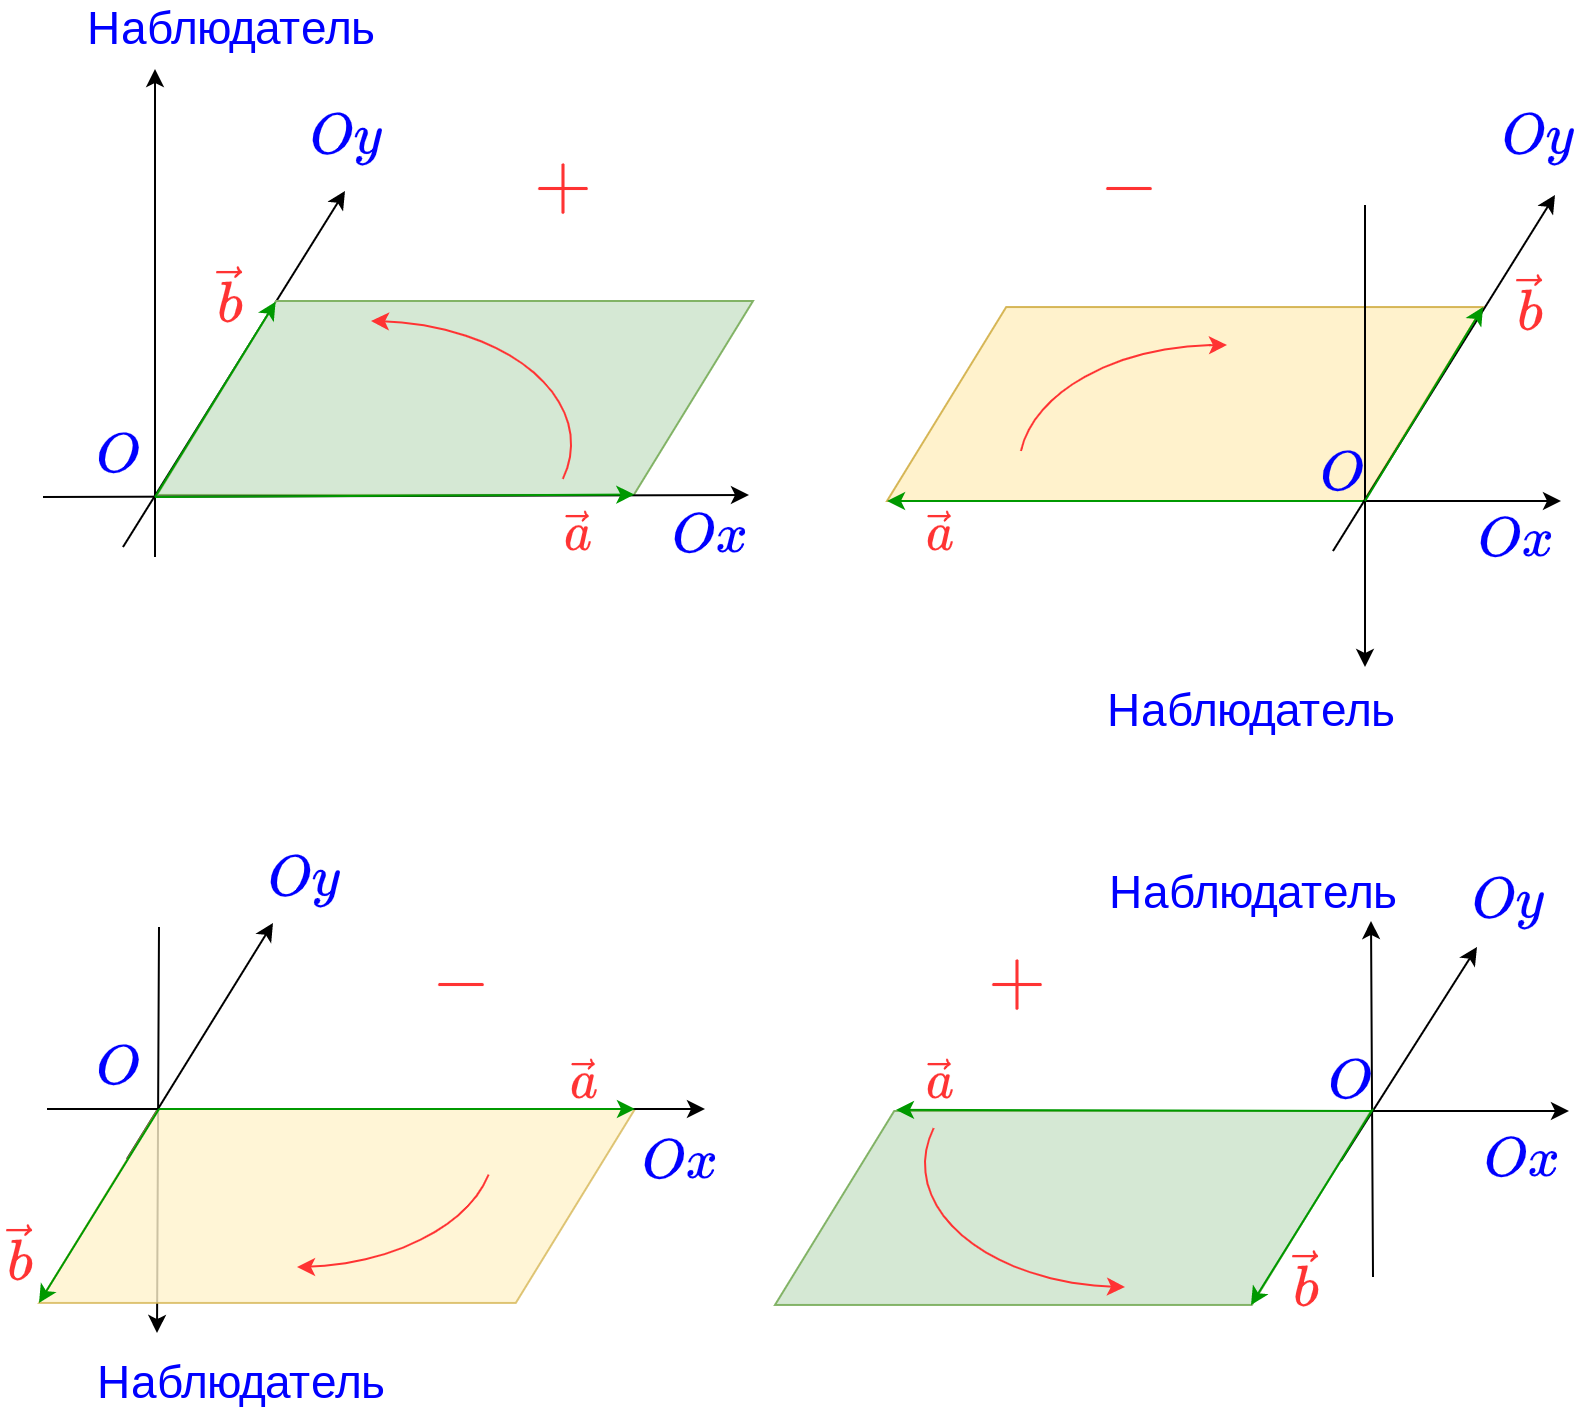
\includegraphics[scale=0.2]{../mult.png}
\end{center}
\caption{произведение $a\cdot b$.}\label{mult}
\end{figure}


\subsection*{Задачи}
\begin{enumerate}
\item Нанести на прямой метки, соответствующие шагам вправо и влево, считая начальной точкой $O$, а все шаги равновеликими (т.е. каждый шаг равен выбранной единице длины). Дойти до точки 5, а затем от точки 5 до точки -5. Записать последовательность шагов с помощью $\pm 1$, предполагая, что шаг вправо записывается как +1, шаг влево --- как -1.
\item Описать в терминах одномерного путешественника операции сложения: $5+3$, $8-4$, $3-5$, $-2-6$. Сколько шагов и в какую сторону он прошел и в каком порядке? Записать в каждом случае путь с помощью $\pm1$ и расставить скобки, объединяя в них указанные слагаемые.
\item \textit{Путь} --- это последовательность единичных шагов, обозначаемых $+1$ (шаг вправо) и $-1$ (шаг влево). Путь может начинаться в любой точке прямой.
Записать пути, соответствующие операциям $-2+7$, $10-5$, $11-2-4$, $-8+3+10$. 
\item Выберем точку $O$ в качестве начала отсчета, затем нанесем на прямую точки, которые получаются в результате отсчета шагов влево и вправо, т.е. точки $\pm1, \pm2, \pm3$ и т.д. Назовем эти точки \textit{целыми}.
\begin{enumerate}[a)]
\item В какой точке окажется путешественник, если он стартует в точке $-3$ и проходит путь $4-1$? Изобразить графически.
\item В какой точке окажется путешественник, если он стартует в точке $1$ и проходит путь $11-4+7$? Изобразить графически.
\end{enumerate}
\item Два пути назовем \textit{эквивалентными}, если, стартуя в одной и той же точке, они и закончатся в одной и той же точке. Эквивалентны ли пути $-2+7$, $10-5$, $11-2-4$, $-8+3+10$?
\item Путь $a$ назовем \textit{обратным} к пути $b$, если, стартовав там, где путь $b$ заканчивается, он повторяет все шаги пути $b$ в обратном порядке и с противоположным знаком (например, путь $1+1+1-1-1-1$ обратен к пути $-1-1-1+1+1+1$). Построить пути, соответствующие операциям $5+3$, $8-4$, $3-5$, $-2-6$, построить обратные к ним пути, выразить обратные пути в виде суммы или разности двух чисел (использовать те же цифры, что у исходного пути).
\item Изобразить ориентированные площади, соответствующие произведениям $3\cdot 5$ и $5\cdot 3$, $(-2)\cdot 6$ и $6\cdot (-2)$, $(-3)\cdot(-4)$ и $(-4)\cdot(-3)$
\end{enumerate}



\begin{comment}
\chapter{2. Соизмеримость отрезков, алгоритм Евклида}
\end{comment}
\newchapter{Соизмеримость отрезков}


\vrezka{<<Дети и наука>>: \href{https://childrenscience.ru/courses/sav/2/}{Урок 2. Соизмеримость и несоизмеримость отрезков}.

Конспект: Глава 1, разделы 1.2 Понятие натурального числа, 1.4 Соизмеримость отрезков, алгоритм Евклида.}

\subsection*{Справочные сведения}

На этот раз у нас имеется два путешественника (кузнечика), каждый из которых имеет свою меру длины (длину шага), соответственно, у каждого из них получаются свои собственные ометки на прямой, расставленные через каждый шаг. Пусть у первого путешественника шаг равен $a$, а у второго --- $b$. Таким образом, первый может придти в точки $\pm a, \pm 2a, \pm 3a$ и т.д., а второй --- в точки $\pm b, \pm 2b, \pm 3b$ и т.д. Точка начала отсчета у них общая --- точка $O$. 

Длины шагов этих путешественников, т.е. числа $a$ и $b$ \textit{соизмеримы}, если существует такая длина $c$ (\textit{общая мера отрезков} $a$ и $b$), которая целое число раз укладывается в том и другом шаге: $a=nc$, $b=mc$. 

\textit{Графический алгоритм Евклида}: о прямоугольника со сторонами $a$ и $b$ отрезают квадраты со стороной, равной меньшей из длин $a$ и $b$, столько раз, сколько возможно (будем называть это <<операцией Евклида>>). К оставшемуся прямоугольнику снова применяют операцию Евклида, и так далее (см. рис. \ref{soizmer}).
\begin{figure}[hbt!]
\begin{center}
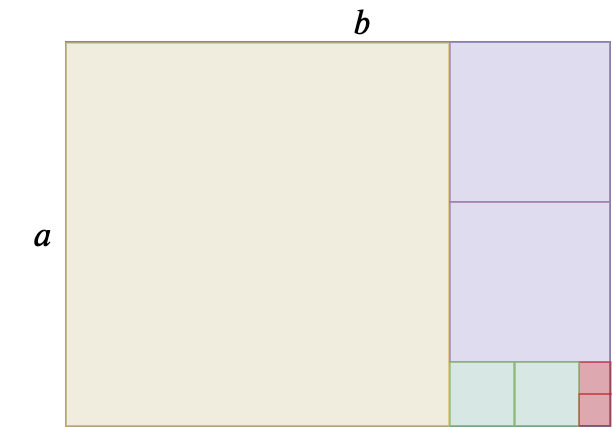
\includegraphics[scale=0.3]{../soizmer.png}
\end{center}
\caption{Графический алгоритм Евклида.}\label{soizmer}
\end{figure}

\textit{Наибольший общий делитель} целых чисел $a$ и $b$ --- это наибольшее целое число, делящее $a$ и $b$. Обозначение: $\gcd(a,b)$. Если $\gcd(a,b)=1$, то числа $a$ и $b$ называются \textit{взаимно простыми} (обозначается так: $a\perp b$).

\subsection*{Задачи}
\begin{enumerate}
\item Найти $\gcd(10,6)$, $\gcd(11,5)$, $\gcd(12,9)$ методом прямоугольников.
\item Сколько и каких шагов должны сделать 10- и 6-шаговые кузнечики, чтобы попасть в точку НОД(10,6)?
\item Доказать, что $a$ и $b$ соизмеримы тогда и только тогда, когда существует отрезок $d$ такой, что отрезки $a$ и $b$ укладываются в нем целое число раз: $d=ka=lb$. Верно ли, что это также равносильно тому, что два путешественника могут встретиться в какой-то точке прямой, отличной от точки $O$?
\item Верно ли, что отрезки $a$ и $b$ соизмеримы тогда и только тогда, когда $a$ и $2b$ соизмеримы?
\item Сколько и каких квадратов получится в результате применения графического алгоритма Евклида к прямоугольнику со сторонами 75 и 21? а со сторонами 324 и 141?
\item Применяя операцию Евклида, прямоугольник разрезали на большой квадрат, два квадрата поменьше и два совсем маленьких. Найти отношение сторон исходного прямоугольника.
\item Доказать, что если стороны прямоугольника соизмеримы, то, применяя операцию Евклида, мы в конце концов разрежем его на квадраты (применить метод бесконечного спуска).
\item Доказать, что если применение графического алгоритма Евклида разрезает прямоугольник на некоторое конечное число квадратов, то стороны прямоугольника соизмеримы, и сторона самого маленького квадрата будет их наибольшей общей мерой.
\item Доказать, что любая общая мера соизмеримых отрезков $a$ и $b$ целое число раз укладывается в наибольшей общей мере отрезков $a$ и $b$.
\item От прямоугольника отрезали квадрат и получили прямоугольник, подобный исходному. Соизмеримы ли стороны исходного прямоугольника? Чему равно отношение его сторон?
\item Докажите, что $\gcd(a,b)$ существует и единственный, если целые $a$ и $b$ не равны одновременно нулю.
\item Докажите, что $\gcd(a,b)=\gcd(a-b,b)=\gcd(r,b)$, где $r$ --- остаток от дееления $a$ на $b$.
\item Найдите наибольшую общую меру отрезков $15/28$ и $6/35$.
\item Какие расстояния можно отложить на прямой, имея шаблоны 6 см и 15 см?
\item Найдите возможные значения а) $\gcd(n,12)$; б) $\gcd(n,n+1)$; в) $\gcd(2n+3,7n+6)$; г) $\gcd(n^2,n+1)$.
\end{enumerate}


\begin{comment}
\chapter{3. Визуальная арифметика}
\end{comment}
\newchapter{Визуальная арифметика}


\vrezka{<<Дети и наука>>: \href{https://childrenscience.ru/courses/sav/3/}{Урок 3. Визуальное представление бинома Ньютона}.

Конспект: Глава 1, раздел 1.3 Визуальные доказательства.}

\subsection*{Справочные сведения}

Теорема Пифагора (см. рис. \ref{pithagor}) и куб суммы (см. рис. \ref{kub}).

\begin{figure}[hbt!]
\begin{center}
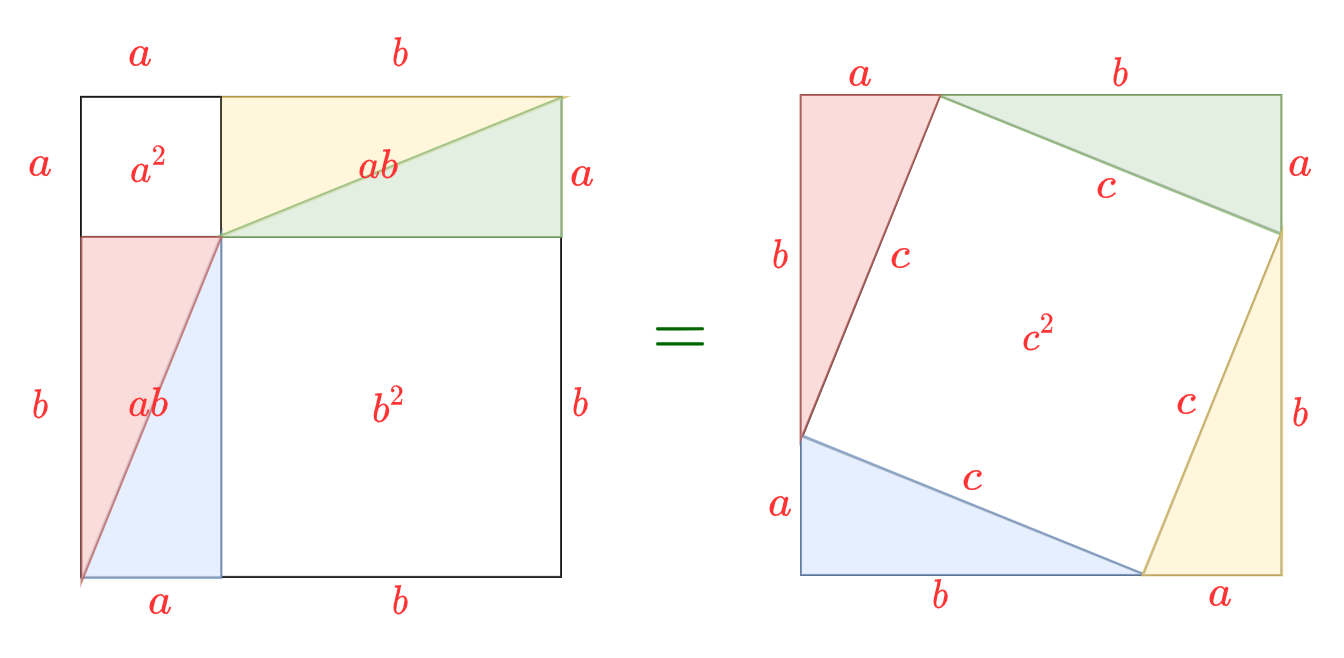
\includegraphics[scale=0.25]{../pithagor.png}
\end{center}
\caption{$(a+b)^2=a^2+2ab+b^2$ и $a^2+b^2=c^2$.}\label{pithagor}
\end{figure}

\begin{figure}[hbt!]
\begin{center}
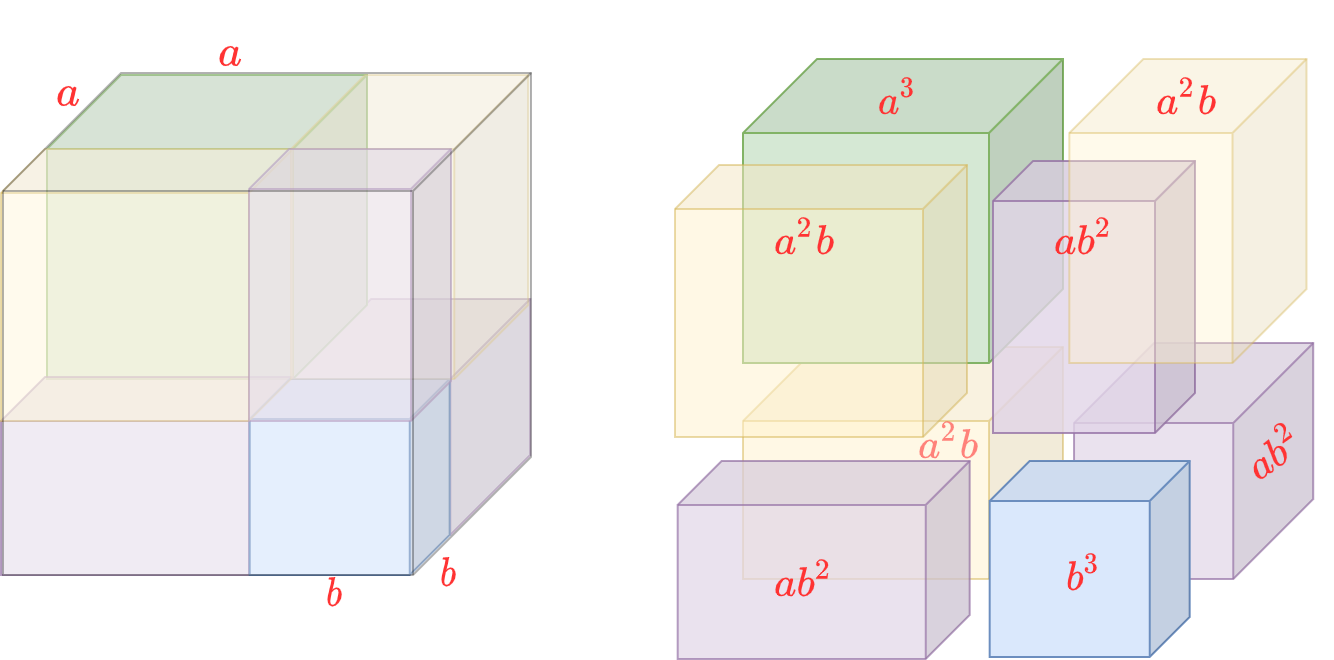
\includegraphics[scale=0.25]{../kub.png}
\end{center}
\caption{$(a+b)^3 = a^3+3a^2b+3ab^2+b^2$.}\label{kub}
\end{figure}



\subsection*{Задачи}
\begin{enumerate}
\item Найти с помощью графического метода сумму подряд идущих нечетных чисел от 1 до $n$, где $n$ --- нечетное.
\item Рассмотрим последовательность уголков (см. рис. \ref{ugolki}). Сколько клеток в $k$-м уголке? Чему равна суммарная площадь первый $k$ уголков?
\begin{figure}[hbt!]
\begin{center}
 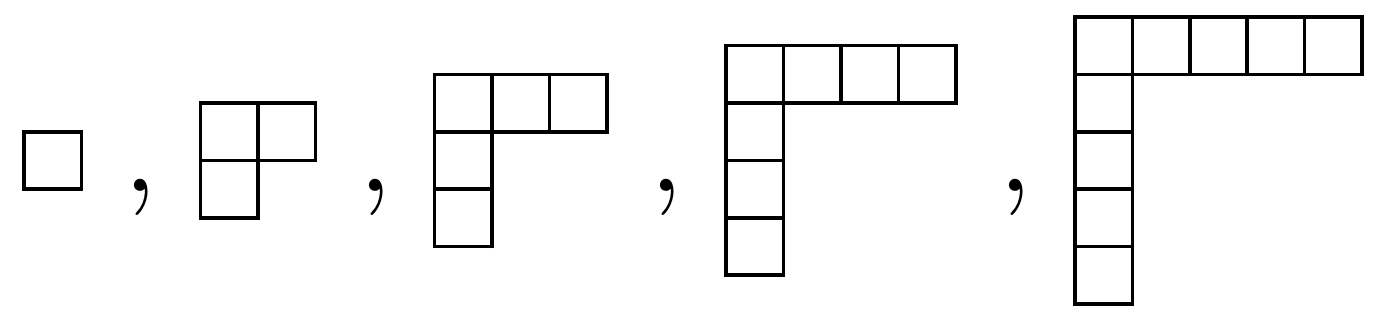
\includegraphics[scale=0.3]{../ugolki.png}
\end{center}
\caption{}\label{ugolki}
\end{figure}
\item Найти графически сумму первых $k$ четных и первых $k$ нечетных чисел.
\item Треугольные числа Диофанта  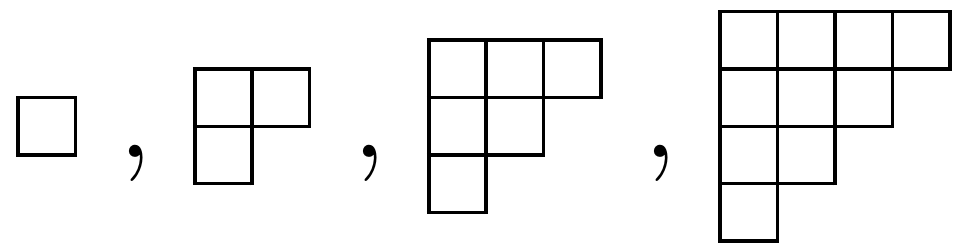
\includegraphics[scale=0.1]{../triangle.png} обозначим по порядку $T_1,T_2,T_3,T_4$ и т.д.
\begin{enumerate}[a)]
\item Сложите из двух последовательных треугольных чисел квадрат.
\item Что получится при сложении $T_n$ с $T_n$?
\item Выразив $T_n$ через $n$, найдите $1+2+\dots+n$.
\item Докажите геометрически, что $T_{n+m}=T_n+T_m+nm$.
\end{enumerate}
\item Докажите геометрически, что $1+2+\dots+(n-1)+n+(n-1)+\dots+2+1=n^2$.
\item Получите геометрически выражение для $(a+b+c)^2$, $(a+b+c)^3$.
\item Объясните равенство на рис. \ref{sumquad} и получите формулу для суммы квадратов $1^2+2^2+3^2+\dots+n^2$.
\begin{figure}[hbt!]
\begin{center}
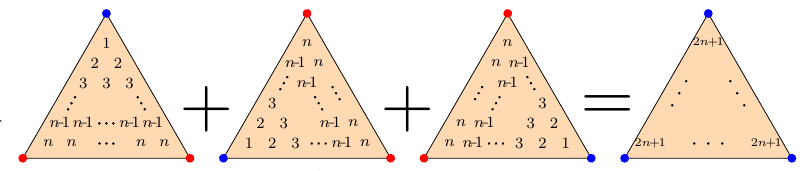
\includegraphics[scale=0.75]{../sumquad.png}
\end{center}
\caption{}\label{sumquad}
\end{figure}

\item С помощью рис. \ref{sumquad2} получите еще один способ найти формулу для суммы квадратов.
\begin{figure}[hbt!]
\begin{center}
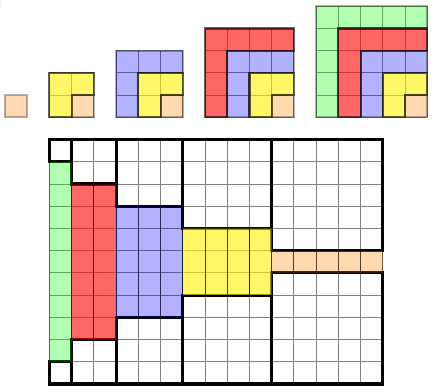
\includegraphics[scale=0.6]{../sumquad2.png}
\end{center}
\caption{}\label{sumquad2}
\end{figure}
\end{enumerate}



\begin{comment}
\chapter{4. Бесконечные суммы}
\end{comment}
\newchapter{Бесконечные суммы}


\vrezka{<<Дети и наука>>: \href{https://childrenscience.ru/courses/sav/4/}{Урок 4. Бесконечные суммы}.
}

\subsection*{Справочные сведения}

В данном разделе мы рассматриваем только суммы \textit{положительных} слагаемых.

Бесконечные суммы с положительными слагаемыми могут быть сходящимися и расходящисмися. Сходимость означает, что найдется такое число, что любой сколь угодно длинный конечный отрезок данной бесконечной суммы меньше этого числа. Например, сумму
$1+1/2^2+1/3^2+1/4^2+\dots$ можно оценивать так:
$$
\frac{1}{2^2}+\frac{1}{3^2}<\frac{1}{2^2}+\frac{1}{2^2}=\frac12,
$$
$$
\frac{1}{4^2}+\frac{1}{5^2}+\frac{1}{6^2}+\frac{1}{7^2}<\frac{1}{4^2}+\frac{1}{4^2}+\frac{1}{4^2}+\frac{1}{4^2}=\frac14,
$$
и т.д. То есть, сумму можно разбить на отрезки длиной 2, 4, 8, 16 и т.д. слагаемых, причем сумма по каждому такому отрезку будет оцениваться сверху дробью $1/2^k$. Остается заметить, что ряд
$$
1+\frac{1}{2}+\frac{1}{4}+\frac{1}{8}+\frac{1}{16}+\dots
$$
сходится. А это легко обнаружить на картинке \ref{geomseq} последовательным делением квадрата $1\times 1$ пополам.
\begin{figure}[hbt]
\begin{center}
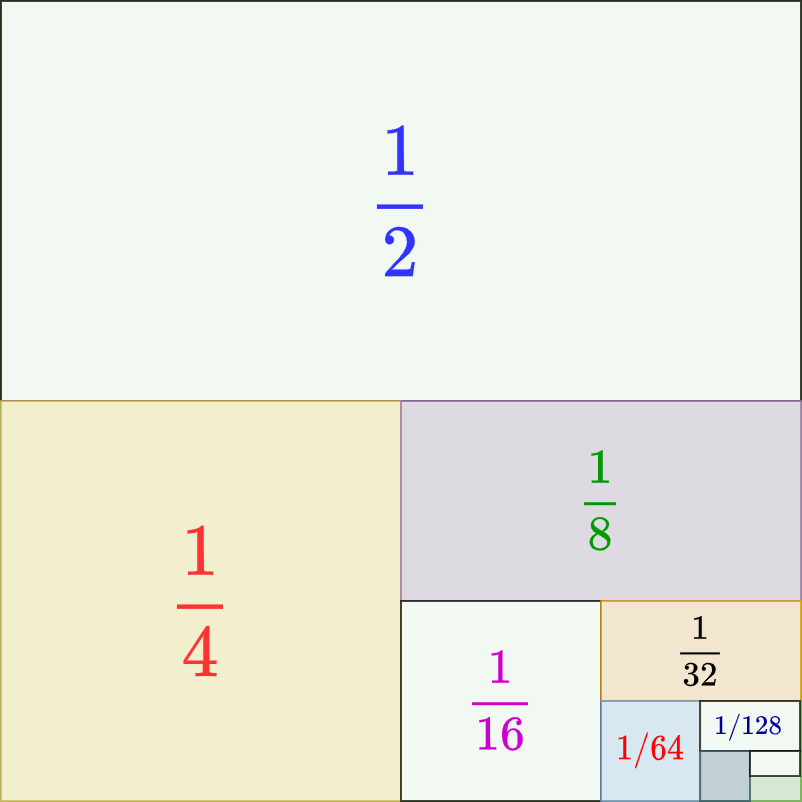
\includegraphics[scale=0.3]{../geomseq.png}
\end{center}
\caption{}\label{geomseq}
\end{figure}
Таким образом, для суммы обратных квдаратов справедлива оценка:
$$
1+1/2^2+1/3^2+1/4^2+\dots \le 1+\frac{1}{2}+\frac{1}{4}+\frac{1}{8}+\frac{1}{16}+\dots \le 2.
$$

Обратно, для некоторых рядов можно найти такую оценку снизу, которая будет заведомо бесконечной, а значит, и сумма исходного ряда также будет бесконечной. Такое верно, например, для гармонического ряда:
$$
1+\frac{1}{2}+\frac{1}{3}+\frac{1}{4}+\frac{1}{5}+\dots \ge 
1+\frac{1}{2}+\frac{1}{4}+\frac{1}{4}+4\cdot\frac{1}{8}+8\cdot\frac{1}{16}+\dots,
$$
а это --- бесконечная сумма одинаковых слагаемых, равных $1/2$ (кроме первого слагаемого). Ясно, что какое бы большой число мы ни выбрали, можно взять столь много раз $1/2$, что их сумма будет больше выбранного числа. А значит, и сумма гармонического ряда равна бесконечности.

\subsection*{Задачи}

\begin{enumerate}
\item Выведите формулу суммы геометрической прогрессии $1+x+x^2+x^3+\dots$ ($0<x<1$) путем домножения этой суммы на $x$. Найти:
\begin{enumerate}[a)]
\item $\displaystyle \frac{1}{10}+\frac{1}{100}+\frac{1}{1000}+\dots$;
\item $\displaystyle 1+0.2+(0.2)^2+(0.2)^3+\dots$;
\item $\displaystyle \frac{1}{0.99}+\frac{1}{0.99^2}+\frac{1}{0.99^3}+\dots$.
\end{enumerate}
\item Исследовать ряды на сходимость:
\begin{enumerate}[a)]
\item $1+1/3+1/5+1/7+\dots$;
\item $1+1/3^2+1/5^2+1/7^2+\dots$;
\item $\displaystyle \frac{1}{1001}+\frac{1}{2001}+\frac{1}{3001}+\dots+\frac{1}{1000n+1}+\dots$;
\item $\displaystyle 1+\frac{1}{2!}+\frac{1}{3!}+\frac{1}{4!}+\dots$;
\item $\displaystyle 1+\frac{2}{3}+\frac{3}{5}+\frac{5}{9}+\dots+\frac{n}{2n-1}+\dots$.
\end{enumerate}
\item Доказать, что если ряды $\displaystyle \sum_na_n^2$ и $\displaystyle \sum_nb_n^2$ сходятся, то сходятся также и ряды:
$$
\sum_na_nb_n,\quad \sum_n(a_n+b_n)^2.
$$
Здесь все $a_n,b_n\ge 0$.
\item Доказать сходимость ряда
$$
a_0+\frac{a_1}{10}+\frac{a_2}{10^2}+\dots+\frac{a_n}{10^n}+\dots,
$$
где $0\le a_n<10$.
\end{enumerate}





\begin{comment}
\chapter{5. Движения прямой: работа с понятием}
\end{comment}
\newchapter[работа с понятием]{Движения прямой:}


\vrezka{<<Дети и наука>>: \href{https://childrenscience.ru/courses/sav/5/}{Урок 5. Начальные представления о движении}.

Конспект: Глава 2, разделы 2.1 Сдвиг, композиция сдвигов, группа и раздел 2.2 Отражение.}

\subsection*{Справочные сведения}

\textit{Движением} называется такое преобразование (прямой, фигуры, плоскости, области пространства и т.д.), которое сохраняет расстояния. Т.е. если между точками $A$ и $B$ расстояние равно $x$, то между точками $A'$ и $B'$, в которые переходят исходные точки $A$ и $B$ при некотором движении, расстояние также будет равно $x$.

На прямой рассматриваются следующие два вида движений:
\begin{itemize}
\item Сдвиг на $x$, когда все точки, как по команде, сдвигаются на число $x$ (если $x>0$, то вправо, а если $x<0$, то влево). Сдвиг на $x$ обозначается за $T_x$. Сдвиг на вектор $AB$ обозначается $T_{AB}$.
\item Отражение относительно точки $O$, когда все точки переходят в симметричные себе относительно точки $O$. Отражение относительно точки $O$ обозначается за $S_O$.
\end{itemize}

Частный случай сдвига --- тождественное движение $\id$, которое ничего не меняет (все точки остаются на своих местах). $\id=T_0$ (сдвиг на нулевой вектор).

Композиция движений $G$ и $Q$ записывается как $G\circ Q$, что означает последовательное применение движений: сначала ко всем точкам прямой применяется движение $Q$, а затем к результату предыдущего движения применяется движение $G$. Композиция движений есть движение.



\subsection*{Задачи}

Пусть на прямой даны 4 точки $A,B,C,D$, поставленные друг за другом с одинаковым шагом (см. рис. \ref{ABCD}).
\begin{figure}[hbt!]
\begin{center}
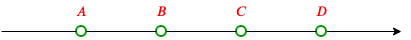
\includegraphics[scale=0.7]{../ABCD.png}
\end{center}
\caption{}\label{ABCD}
\end{figure}

\begin{enumerate}
\item Куда перейдет точка $A$ при отражении $S_B$?
\item Куда перейдут точки $B,C,D$ при преобразовании $T_{AB}\circ T_{CA}$?
\item Куда перейдут точки $A,B,C$ при преобразовании $S_C\circ T_{AB}$?
\item Какое движение переводит $A$ в $C$ и $B$ в $D$?
\item Существует ли движение, которое переводит $A$ в $B$ и $B$ в $D$?
\item Опишите все движения, которые переводят $A$ в $C$, используя только буквы $A,B,C,D$ и обозначения сдвига и отражения.
\end{enumerate}




\begin{comment}
\chapter{6. Движения прямой: классификация}
\end{comment}
\newchapter[классификация]{Движения прямой:}


\vrezka{<<Дети и наука>>: \href{https://childrenscience.ru/courses/sav/6/}{Урок 6. Классификация движений прямой}.

Конспект: Глава 2, раздел 2.4 Теорема о гвоздях, аналог теоремы Шаля.}

\subsection*{Справочные сведения}

Всякое движение прямой --- это либо сдвиг, либо отражение. При этом любое движение --- это либо одно отражение, либо композиция двух отражений.

Всякое движение прямой есть \textit{взаимно однозначное соответствие} точек прямой, т.е. оно переводит разные точки в разные, и какова бы ни была точка прямой, найдется точка, переходящая в нее под действием движения.

\textit{Обратное движение} для дивжения $G$ --- это такое движение $G^{-1}$, что $G\circ G^{-1}=G^{-1}\circ G=\id$.

Обращение композиции: $(G\circ Q)^{-1} = Q^{-1}\circ G^{-1}$.

\subsection*{Задачи}

Введем координату на прямой, отметим там точки с целыми координатами: $\dots,-2,-1,0,1,2,\dots$. Через $S_n$ обозначим отражение относительно точки $n$, через $T_n$ --- сдвиг на число $n$.
\begin{enumerate}
\item Известно, что при некотором преобразовании $G$ точка $0$ переходит в $2$, а $2$ --- в $3$. Может ли оно быть движением? Каким?
\item Известно, что при некотором преобразовании $G$ точка $0$ переходит в $3$, а $2$ --- в $1$. Может ли оно быть движением? Каким?
\item Известно, что при некотором преобразовании $G$ точка $0$ переходит в $2$, а при обратном преобразовании $G^{-1}$ точка $3$ переходит в $-1$. Может ли $G$ быть движением? Каким?
\item Дано движение $G$. Известно, что $G^{-1}(0)=1$ и при этом у $G^{-1}$ нет неподвижных точек. Чему равно $G$?
\item Назовем \textit{четностью движения} прямой четность количества отражений, с помощью которых это движение может быть выражено. Какова четность следующих движений: $S_0$, $T_x$, $T_x\circ T_y$, $S_0\circ T_x$, $S_0\circ S_1\circ T_x\circ T_y$, $T_x^{-1}$, $S_9^{-1}$, $S_0\circ S_1\circ\dots\circ S_n$?
\item Доказать, что
\begin{enumerate}[a)]
\item Четность обратного движения  $G^{-1}$ совпадает с четностью исходного движения $G$.
\item Четность композиции движений равна сумме четностей (по модулю 2) компонентов.
\item Четность движения не зависит от его представления в виде композиций каких-либо движений.
\end{enumerate}
\end{enumerate}






\begin{comment}
\chapter{7. Движения прямой: таблица композиций}
\end{comment}
\newchapter[таблица композиций]{Движения прямой:}


\vrezka{<<Дети и наука>>: \href{https://childrenscience.ru/courses/sav/7/}{Урок 7. Таблица композиций движений прямой}.

Конспект: Глава 2, раздел 2.3 Таблица композиций движений прямой.}

\subsection*{Справочные сведения}


Таблица композиций отражений и сдвигов:\index{Группа!движений прямой}
\begin{center}
\begin{tabular}{c|c|c|}
  & $T_a$ & $S_O$ \\
 \hline
$T_b$ & $T_{a+b}$ & $S_{O+b/2}$ \\
 \hline
$S_C$ & $S_{C-a/2}$ & $T_{2OC}$ \\
\hline
\end{tabular}
\end{center}

Таблицу композиций следует читать слева наверх, т.е. если в левом столбце стоит движение $F$, а в верхней строке --- движение $G$, то в соответствующей ячейке стоит композиция $F\circ G$.


\subsection*{Задачи}

Введем координату на прямой, отметим там точки с целыми координатами: $\dots,-2,-1,0,1,2,\dots$. Через $S_n$ обозначим отражение относительно точки $n$, через $T_n$ --- сдвиг на число $n$.
\begin{enumerate}
\item Какое движение получится при композиции
\begin{enumerate}[a)]
\item $S_0\circ S_1$?
\item $S_0\circ S_1\circ S_2$?
\item $S_0\circ S_2\circ S_1$?
\end{enumerate}
\item Построить сдвиг на 7 единиц вправо с помощью композиции двух отражений.
\item Каким движением является следующая композиция?
$$
S_{n}\circ S_{n-1}\circ \dots\circ S_{1}\circ S_0.
$$
Ответ получить в зависимости от четности $n$.
\item При каких $n$ сдвиг $T_n$ выражается в виде композиций $S_0$ и $S_1$?
\item При каких $n$ сдвиг $S_n$ выражается в виде композиций $S_0$ и $S_1$?
\item Пусть $G$ и $Q$ --- два движения прямой, причем $G\circ Q=Q\circ G$ и $G\ne Q$. Какими могут быть $G$ и $Q$?
\item Пусть $G$ и $Q$ --- два движения прямой, причем $G\circ Q=\id$ и $G\ne Q$. Какими могут быть $G$ и $Q$?
\item Вывести равенства $S_C\circ T_a = S_{C-a/2}$ и $T_b\circ S_O = S_{O+b/2}$ из соотношения $S_C\circ S_O=T_{2OC}$ алгебраическим путем.
\item Доказать, что никакая композиция движений $S_n$ и $T_m$ с целыми индексами $n,m$ не может быть равна сдвигу $T_x$ с нецелым $x$ и отражению $S_y$ с неполуцелым $y$.
\end{enumerate}



\begin{comment}
\chapter{8. Движения окружности: классификация}
\end{comment}
\newchapter[классификация]{Движения окружности:}


\vrezka{<<Дети и наука>>: \href{https://childrenscience.ru/courses/sav/8/}{Урок 8. Движения окружжности}.

Конспект: Глава 3, раздел 3.1 Движения окружности, раздел 3.2 Группа движений окружности, теорема Шаля.}

\subsection*{Справочные сведения}

Чтобы корректно говорить о движениях в криволинейном пространстве, нужно сначала договориться о метрике на нем. \textit{Расстояние} (метрика) между двумя точка окружности --- это длина меньшей из дуг данной окружности, соединяющих эти точки. Таким образом, движение окружности по определению должно сохранять длину дуги, переводя точки окружности в точки этой же окружности.

В отличие от прямой, на окружности расстояния имеют максимально допустимное значение, а именно, половину длины этой окружности. На масимальном расстоянии находятся диаметрально противоположные точки.

Движения на окружности являются:
\begin{itemize}
\item \textit{Отражение относительно диаметра} (произвольного). Отражение обозначается $S_l$, где $l$ --- диаметр. Если на окружности зафиксировано нулевое положение диаметра, то любой диаметр можно определить через угол наклона относительно улевого диаметра (угол откладывается против часовой стрелки). Если диаметр $l$ имеет наклон $\ph$ относительно нулевого диаметра ($0\le\ph<\pi$), то отражение относительно данного диаметра мы также записваем как $S_\ph$.
\item \textit{Поворот окружности} относительно ее центра. Поворот обозначается $R_\ph$, где $\ph$ --- угол поворота относительно центра окружности, осуществляемый против часовой стрелки, $0\le\ph<2\pi$.
\end{itemize}
В обоих случаях можно рассматривать и другие значения угла $\ph$, приводя его по модулю $\pi$ в случае отражений и по модулю $2\pi$ в случае поворотов, т.к. наклон диаметра на угол $\phi\pm\pi$ приводит к диаметру с углом $\ph$, а поворот на угол $\pi\pm2\pi$ --- это поворот на угол $\ph$.

Углы измеряются в радианах. 1 радиан --- это угол, соответствующей дуге, длина которой равна радиусу окружности. Угол в $180^o$, соответствующий дуге, равной половине длины окружности, он же --- развернутый угол, --- имеет радианную меру, равную числу $\pi$. Если окружность имеет радиус, равный 1, то мера угла в радианах численно совпадает с длиной соответствующей этому углу дуги данной окружности.

Частным случаем поворота является \textit{тождественное движение} $\id$, оставляющее все точки окружности на месте. $\id=R_0=R_{2\pi k}$.

Других движений окружности не существует (теорема Шаля). Как и в случае прямой, любое движение окружности можно представить как композицию одного или двух отражений.

\subsection*{Задачи}

\begin{enumerate}
\item Доказать, что $\pi>3$.
\item Пусть $G$ --- движение окружности. Сколько у $G$ может быть неподвижных точек (имеется ввиду общее количество, найдите все возможные варианты)?
\item Пусть $G$ --- движение окружности. Известно, что $G(A)=A$ и $G(B)\ne B$. Какой вид может иметь $G$?
\item Пусть диаметры $l$ и $k$ перпендикулярны. Найдите $S_l\circ S_k$.
\item Известно, что точка $A$ переходит при движении $G$ окружности в точку $A'$, диаметрально противоположную точке $A$. Каким может быть движение $G$?
\item Движение назовем \textit{четным}, если оно является композицией двух отражений, а в противном случае --- \textit{нечетным}. Верно ли, что:
\begin{enumerate}[a)]
\item Композиция четных движений --- четное движение, композиция двух нечетных движений --- четное движение, композиция четного движения с нечетным движением --- нечетное движение?
\item $G$ четно тогда и только тогда, когда $G^{-1}$ нечетно?
\end{enumerate}
\end{enumerate}





\begin{comment}
\chapter{9. Движения окружности: таблица композиций}
\end{comment}
\newchapter[таблица композиций]{Движения окружности:}


\vrezka{<<Дети и наука>>: \href{https://childrenscience.ru/courses/sav/9/}{Урок 9. Таблица умножения движений окружности}.

Конспект: Глава 3, раздел 3.2 Группа движений окружности, теорема Шаля.}

\subsection*{Справочные сведения}

Таблица композиций движений окружности:
\begin{center}
\begin{tabular}{c|c|c|}
  & $R_\al$ & $S_\psi$ \\
 \hline
$R_\be$ & $R_{\al+\be}$ & $S_{\psi+\be/2}$ \\
 \hline
$S_\ph$ & $S_{\ph-\al/2}$ & $R_{2(\ph-\psi)}$ \\
\hline
\end{tabular}
\end{center}

Таблицу композиций следует читать слева наверх, т.е. если в левом столбце стоит движение $F$, а в верхней строке --- движение $G$, то в соответствующей ячейке стоит композиция $F\circ G$.

\subsection*{Задачи}
\begin{enumerate}
\item Центральная симметрия --- это какое движение?
\item Композицией каких отражений можно выразить центральную симметрию?
\item С помощью отражения относительно оси $Ox$ (горизонтальной оси) и вращений выразить отражение относительно оси $Oy$ (вертикальной оси).
\item Возьмем некоторый угол $\ph>0$. Найдите:
\begin{enumerate}[a)]
\item $S_0\circ S_\ph$;
\item $S_0\circ S_\ph\circ S_{2\ph}$;
\item $S_0\circ S_{2\ph}\circ S_{\ph}$;
\item $\displaystyle S_0\circ S_\ph\circ S_{2\ph}\circ S_{3\ph}\circ\dots\circ S_{n\ph}$.
\item Чему равно последнее выражение, если $\ph=\pi/2$, $\ph=\pi$, $\pi=2\pi$?
\end{enumerate}
\item Построить поворот на угол $90^o$ при помощи двух отражений.
\item При каких $n$ поворот на угол $n\ph$ выражается в виде композиций $S_0$ и $S_\ph$?
\item Пусть $G$ и $Q$ --- движения окружности, причем $G\circ Q=Q\circ G$. Какими могут быть $G$ и $Q$?
\item Пусть $G$ и $Q$ --- движения окружности, причем $G\circ Q=\id$. Какими могут быть $G$ и $Q$?
\end{enumerate}







\begin{comment}
\chapter{10. Конечные подгруппы движений прямой и окружности}
\end{comment}
\newchapter[ прямой и окружности]{Конечные подгруппы движений}


\vrezka{<<Дети и наука>>: \href{https://childrenscience.ru/courses/sav/10/}{Урок 10. Конечные подгруппы движений прямой и окружности}.

Конспект: Глава 2, раздел 2.5 Все конечные подгруппы движений прямой, раздел 5.3 Подгруппы движений окружности.}

\subsection*{Справочные сведения}

Все движения прямой и все движения окружности образуют группы с операцией композиции. Напомним определение группы.
Пусть на множестве $G$ задана операция $\circ$. Множество $G$ с данной операцией называется \textit{группой}, если:
\begin{enumerate}[G1]
\setcounter{enumi}{-1}
\item $a\circ b\in G$ для всех $a,b\in G$ (группоид);
\item для любых $a,b,c\in G$ имеем тождество $(a\circ b)\circ c=a\circ (b\circ c)$ (ассоциативность);
\item существует элемент $\id\in G$ такой, что $a\circ \id=\id\circ a=a$ для всех $a\in G$ (единица);
\item для всякого $a\in G$ существует обратный элемент $a^{-1}\in G$ такой, что $a\circ a^{-1}=a^{-1}\circ a=\id$ (обратный элемент).
\end{enumerate}

Кроме того, группа называется \textit{абелевой} (или \textit{коммутативной}), если $a\circ b=b\circ a$ для всех $a,b\in G$. Количество элементов в группе называется ее \textbf{порядком}.

\textit{Конечная подгруппа} может быть определена следующим образом: это --- \textit{конечное подмножество группы, замкнутое относительно групповой операции}. Такого определения достаточно, чтобы вывести из него тот факт, что данное подмножество само по себе является группой, т.е. содержит единицу (исходной группы), обратные элементы, а также удовлетворяет требованию ассоциативности операции (т.к. операция та же самая).

Всякая конечная подгруппа группы движений прямой имеет вид либо $\{\id\}$, либо $\{\id,S_A\}$, где $A$ --- некоторая точка прямой.

Всякая конечная подгруппа группы движений окружности имеет один из видов:
\begin{enumerate}
\item тривиальная подгруппа $\{\id\}$;
\item группа поворотов правильного $n$-угольника (включая случай вырожденного 2-угольника);
\item подгруппа одного отражения $\{\id,S_\ph\}$;
\item группа движений правильного $n$-угольника (включает повороты, совмещающие углы многоугольника, и отражения относительно осей, проходящих через его вершины и центр окружности).
\end{enumerate}


\subsection*{Задачи}

\begin{enumerate}
\item Выпишите все конечные подгруппы группы движений окружности порядка не выше 6, содержащие отражение $S_0$ (относительно горизонтальной оси).
\item Какова группа движений правильного треугольника, квдарата, пятиугольника?
\item Пусть задан правильный треугольник $ABC$ с осями симметрии $a,b,c$ и центром $O$. Заполните таблицу композиций движений данного треугольника:
\begin{table}[htb!]\begin{center}
\begin{tabular}{c||c|c|c||c|c|c|}
             & $\id$        & $R_{2\pi/3}$ & $R_{4\pi/3}$ & $S_a$        & $S_b$        & $S_c$  \\
\hline\hline
$\id$        & \phantom{$R_{2\pi/3}$} & \phantom{$R_{2\pi/3}$} & \phantom{$R_{2\pi/3}$} & \phantom{$R_{2\pi/3}$} & \phantom{$R_{2\pi/3}$} & \phantom{$R_{2\pi/3}$} \\  \hline
$R_{2\pi/3}$ &  &  &  &  &  &  \\  \hline
$R_{4\pi/3}$ &  &  &  &  &  &  \\  \hline
$S_A$        &  &  &  &  &  &  \\  \hline
$S_B$        &  &  &  &  &  &  \\  \hline
$S_C$        &  &  &  &  &  &  \\  \hline
\end{tabular}
\end{center}\end{table}

Таблицу композиций следует читать слева наверх, т.е. если в левом столбце стоит движение $F$, а в верхней строке --- движение $G$, то в соответствующей ячейке стоит композиция $F\circ G$.
\end{enumerate}



%%%%%%%%%%%%%%%%%%%%%%%%%%%%%%%%%%%%%%%%%%%%%%%%%%%%%%%%%%%%%%%%%%%%%%%%%%%%%%%%%%%%%%%%%%%%%%%
%%%%%%%%%%%%%%%     ОСТАТКИ И ДЕЛИМОСТЬ ЦЕЛЫХ ЧИСЕЛ     %%%%%%%%%%%%%%%%%%%%%%%%%%%%%%%%%%%%%%%
%%%%%%%%%%%%%%%%%%%%%%%%%%%%%%%  ОТА  %%%%%%%%%%%%%%%%%%%%%%%%%%%%%%%%%%%%%%%%%%%%%%%%%%%%%%%%%
%%%%%%%%%%%%%%%%%%%%%%%%%%%%%%%%%%%%%%%%%%%%%%%%%%%%%%%%%%%%%%%%%%%%%%%%%%%%%%%%%%%%%%%%%%%%%%%



\begin{comment}
\chapter{11. Арифметика остатков}
\end{comment}
\newchapter{Арифметика остатков}


\vrezka{<<Дети и наука>>: \href{https://childrenscience.ru/courses/sav/11/}{Урок 11. Введение в арифметику остатков}.

Конспект: Глава 8, раздел 8.1 Арифметика остатков.}

\subsection*{Справочные сведения}

Посмотрим на шкалу целых чисел $0,\pm1,\pm2,\dots$ через некоторый трафарет. Этот трафарет является непрозрачной полоской, в которой проделаны дырки с шагом $m$ друг от друга (где $m$ --- целое положительное число). Например, пусть $m=7$, тогда если в одной дырке мы видим число 0, то в другой, справа от нее, --- число 7, а слева --- $-7$. Если мы сместим трафарет вправо на единицу, то увидим числа $-6$, 1 и 8, еще сдвинем --- числа $-5$, 2 и 9, и т.д.  

Таким образом, в массиве всех целых чисел мы сможем выделять такие числа, которые связаны друг с другом через этот трафарет. Например, все числа кратные 7, т.е. $0,\pm7,\pm14,\dots$. В другой класс войдут все числа, смещенные от них на 1 вправо, т.е. $1,\pm7+1,\pm14+1,\dots$. Эти классы называются \textit{классами вычетов по модулю} $m$.

Если класс содержит число 0, то все числа из данного класса кратны шагу трафарета, т.е. модулю $m$. Действительно, ведь это числа $0,\pm m,\pm 2m$ и т.д. Если класс не содержит нуля, то все числа в нем имеют слева соседа из нулевого класса на одном и том же расстоянии, т.к. это числа вида $k,k\pm m,k\pm 2m,\dots$, где $0<k<m$. Число $k$ является остатком от деления таких чисел на модуль $m$. Между классами и остатками от деления существует взаимно однозначное соответствие.

Простой иллюстрацией из жизни является пример с днями недели. Все понедельники отстоят друг от друга на кратное 7 число дней. Поэтому на шкале дней их можно увидеть через трафарет с шагом 7. Аналогично --- все вторники, среды, четверги, пятницы, субботы и воскресенья. Если воскресенье обозначить за 0, понедельник --- за 1, и т.д., то для любой даты можно определить ее класс, он же --- остаток отделения на 7, т.е. день недели.

Как только мы отождествляем целые числа, входящие в один класс, их арифметика становится \textit{модульной}. Это значит, что арифметические операции мы выполняем с точностью до класса. Так, если сложить $2+5$, то в обычной арифметике мы получим число 7, но оно находится в том же классе, что и число 0 по модулю $m=7$, поэтому в модульной арифметике $2+5=0\mod 7$. Проще говоря, в модульной арифметике мы всякий раз \textit{вычитаем} максимально возможную часть числа, кратную модулю, и оставляем лишь \textit{остаток} от деления на модуль. Поэтому она и называется арифметикой остатков.

\begin{figure}[hbt!]
\begin{center}
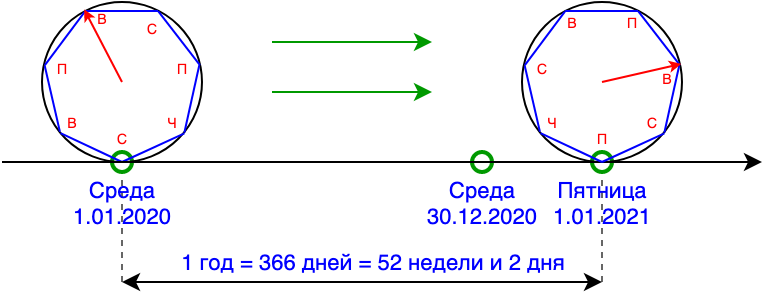
\includegraphics[scale=0.4]{../weekdays.png}
\end{center}
\caption{Арифметика остатков по модулю 7.}\label{weekdays}
\end{figure}

Попадание чисел $a$ и $b$ в один класс по модулю $m$ обозначается так: $a\equiv b\mod m$. Формально это означает, что $a-b=km$ при некотором целом $k$.


Если $a$ делится на $b$ (формально: существует целое $k$ такое, что $a=kb$), то пишут $a\vdots b$, это равносильно записи $b|a$ ($b$ делит $a$). Частный случай: $0\vdots x$ и $x|0$ при любом целом $x$.

\subsection*{Задачи}

\begin{enumerate}
\item Отметить на числовой оси целые числа, которые при делении на 7 дают остаток 2 (на рисунке должны поместиться числа от -20 до 20).
\item Книги на столе пытались связывать в пачки по 2, по 3, по 4 и по 5 книг, и каждый раз оставалась одна лишняя. Сколько книг было на столе? (Известно, что их было не больше 100.)
\item Одному брату 6 лет, другому --- 10. Значит, сумма из возрастов четная. Какой она будет в следующем году?
\item Если сегодня понедельник, то какой день недели будет через 10 дней, через 90 дней, через 2 года (рассмотреть случай без високосных лет и с високосным годом)?
\item Найти день недели через месяц, квартал, полгода и год, отправляясь от текущей даты.
\item Поезд Москва--Владивосток отправляется из Москвы в 7:00 и находится в пути 166 часов. Определите время прибытия (московское) поезда во Владивосток.
\item Построить таблицы сложения  для модулей: 2,3,4,5,6,10,11.
\item Найти число, которое при делении на 2 даёт остаток 1, при
делении на 3 остаток 2, при делении на 4 остаток 3, при делении
на 5 остаток 4, при делении на 6 остаток 5 и при делении на 7 даёт
остаток 6.

\item Верно ли, что а) если $n\vdots k$ и $k\vdots n$, то $n=\pm k$; б) если $a|b$ и $b|c$, то $a|c$; в) если $b\vdots a$ и $c\vdots a$, но $d\not\vdots a$, то $(b+c)\vdots a$, но $(b+d)\not\vdots a$; г) если $a$ и $b$ не делятся на $c$, то $ab$ не делится на $c^2$?

\item Что означает запись $a\equiv b\pmod 0$?

\item Обозначим за $\oplus$ сложение по модулю 2, т.е. $a\oplus b = a+b\pmod 2$, если $a,b\in\{0,1\}$. Для битовых последовательностей эта операция применяется попозиционно (например, $110\oplus 101 = 011$).

Алиса и Боб придумали следующий алгоритм шифрования. Каждый из них сгенерил случайную последовательность длины $n$: $A$ и $B$ соответственно. Алиса передает Бобу сообщение $m$ длиной в $n$ битов следующим способом: она отправляет ему сообщение $m_1=m\oplus A$, в ответ Боб отправляет ей $m_2=m_1\oplus B$, затем Алиса отправляет Бобу $m_3=m_2+A$.

Как Боб сможет прочесть сообщение $m$, зная алгоритм и сообщение $m_3$? Как Ева, перехватившая сообщения $m_1,m_2,m_3$, сможет прочесть исходное сообщение $m$ ?

\end{enumerate}




\begin{comment}
\chapter{12. Таблицы умножения остатков}
\end{comment}
\newchapter{Таблицы умножения остатков}


\vrezka{<<Дети и наука>>: \href{https://childrenscience.ru/courses/sav/12/}{Урок 12. Таблицы умножения остатков}.

Конспект: Глава 8, раздел 8.1 Арифметика остатков, раздел 8.2 Свойства арифметики остатков.}

\subsection*{Справочные сведения}

\begin{wrapfigure}{r}{0.21\textwidth}
\includegraphics[width=0.21\textwidth]{mod5mult.png}
\caption{Умножение по модулю 5.}\label{mod5mult}
\end{wrapfigure}
Умножение остатков производится также по модулю $m$, т.е. после умножения отбрасываем часть, кратную $m$, и оставляем остаток от деления на $m$ (см. рис. \ref{mod5mult}).

Таблица умножения по модулю $m$ обладает следующими свойствами:
\begin{itemize}
\item Она центрально симметрична (на картинке \ref{mod5mult} мы убрали строку и столбец, соответствующие умножению на ноль).
\item Если модуль --- простое число, то нулей в таблице нет (кроме тривиальных строк и столбца).
\end{itemize}


\subsection*{Задачи}

\begin{enumerate}
\item Целое положительное число увеличили на 1. Могла ли сумма
его цифр (а) возрасти на 8? (б)Уменьшиться на 8? (в) Уменьшиться
на 10?
\item Какие остатки может давать точный квадрат при делении на 4?
\item Последняя цифра точного квадрата равна 6. Доказать, что его
предпоследняя цифра нечётна.
\item Остаток от деления простого числа на 30 --- простое число или 1. Почему?
\item Какое наибольшее число различных целых чисел можно выбрать, если требуется, чтобы сумма и разность любых двух из них не делились на 15?
\item На какую цифру оканчивается число $33^{77}+77^{33}$?
\item Могут ли среди $m$ последовательных целых чисел какие-то два иметь равные остатки от
деления на $m$?
\item Пусть $5x\equiv 6\pmod 8$. Найти $x$.
\item Найти последнюю цифру $7^{100}$, $7^{1942}$.
\item Пусть $a \equiv b \pmod m$, $c \equiv d \pmod m$. Докажите, что сравнения по одному и тому же модулю
\begin{enumerate}[a)]
\item можно складывать и вычитать: $a + c \equiv b + d \pmod m$, $a - c \equiv b - d \pmod m$;
\item можно перемножать: $ac \equiv bd \pmod m$;
\item можно возводить в натуральную степень $n$: $a^n \equiv b^n \pmod m$;
\item можно домножать на любое целое число $k$: $ka \equiv kb \pmod m$.
\end{enumerate}
\item Найдите остаток от деления \textbf{а)} числа $1 + 31 + 331 + \dots + 3333333331$ на $3$; \textbf{б)} $6100$ на $7$.
\item Найдите остаток от деления числа $1 - 11 + 111 - 1111 + \dots - 1111111111$ на $9$.
\item Найдите остаток от деления \textbf{а)} $10!$ на $11$; \textbf{б)} $11!$ на $12$.
\item \textbf{а)} Какой цифрой оканчивается $8^{18}$? \textbf{б)} При каких натуральных $k$ число $2^k-1$ кратно $7$?
\item Найдите три последние цифры числа $1999^{2000}$.
\item Найти \textbf{а)} $3^{31}\pmod 7$, \textbf{б)} $2^{35}\pmod 7$, \textbf{в)} $128^{129}\pmod {17}$.
\item Докажите, что \textbf{а)} $30^{99} + 61^{100}$ делится на 31; \textbf{б)} $43^{95} + 57^{95}$ делится на 100.
\item Докажите, что $1^n + 2^n + \dots + (n - 1)^n$ делится на $n$ при нечётном $n$.
\item Числа $x$ и $y$ целые, причем $x^2 + y^2$ делится на 3. Докажите, что $x$ и $y$ делятся на 3.
\item Какие целые числа дают при делении на 3 остаток 2, а при делении на 5 --- остаток 3?
\item Докажите, что остаток от деления простого числа на 30 есть или простое число или 1.
\item (a) Квадрат целого положительного числа оканчивается на ту
же цифру, что и само число. Что это за цифра? (Указать все возможности.) (б) Квадрат целого положительного числа оканчивается на те же две цифры, что и само число. Что это за цифры?
(Указать все возможности.) (в) Пятая степень числа оканчивается
на ту же цифру, что и само число. Почему? Для каких ещё степеней
это верно?
\item Доказать, что для любого целого a число 10a даёт при делении
на 9 тот же остаток, что и само a.
\item Доказать, что число и его сумма цифр дают одинаковые остатки при делении на 3 и 9.
\item *Сколько есть способов записать 2018 как сумму натуральных слагаемых, любые два из
которых равны или различаются на 1? (Способы лишь с разным порядком слагаемых считаем равными.)
\item *Докажите, что из любых $n$ целых чисел всегда можно выбрать несколько, сумма которых
делится на $n$ (или одно число, делящееся на $n$).
\end{enumerate}





\begin{comment}
\chapter{13. Умножение по простому модулю}
\end{comment}
\newchapter{Умножение по простому модулю}


\vrezka{<<Дети и наука>>: \href{https://childrenscience.ru/courses/sav/13/}{Урок 13. Основная теорема арифметики. Часть 1}.

Конспект: Глава 4, раздел 4.2 Кузнечик НОД и алгоритм Евклида, раздел 4.3 Простые числа и ОТА, Глава 8, раздел 8.1 Арифметика остатков, раздел 8.2 Свойства арифметики остатков.}

\subsection*{Справочные сведения}

Для произвольной строки (столбца) таблица умножения остатков по модулю $m$ эквивалентны следующие утверждения:
\begin{itemize}
\item В строке (столбце) отсутствует ноль;
\item Номер строки (столбца) взаимно прост с модулем $m$;
\item В строке (столбце) встречаются все числа от 1 до $m-1$;
\item В строке (столбце) встречается 1.
\end{itemize}

Натуральное число $p$ --- \textit{простое}, если оно имеет ровно два положительных делителя (1 и $p$).

Таблица умножения остатков по простому модулю $p$ не содержит нулей (кроме строки и столбца с умножением на ноль) и все строки и столбцы являются перестановками множества $\{1,\dots,p-1\}$.

В таблице умножения остатков по простому модулю $p$ номер $k$ любой строки взаимно прост с модулем: $\gcd(k,p)=1$. Отсюда следует, что при некоторых целых $n,m$ имеем $mp-nk=1$, а по модулю $p$ это равенство принимает вид $nk\equiv 1$, т.е. число $n$ обратно к $k$ по модулю $p$. Таково же и число $n\mod p$. Иначе говоря, равенство $mp-nk=1$ позволяет найти обратный к остатку $k$ остаток по модулю $p$.

Коэффициенты $n,m$ можно найти методом цепных дробей. Например, пусть $p=101$, $k=77$. Найдем обратный к нему остаток. Для этого используем цепную дробь
$$
\frac{101}{77} = 1+\frac{1}{3+\frac{1}{5-\frac{1}{5}}}\approx
1+\frac{1}{3+\frac{1}{5}}=\frac{21}{16}.
$$
откуда видим, что $77\cdot 21-101\cdot 16=1$. Поэтому $77\cdot 21\equiv 1\pmod{101}$, т.е. остаток 21 обратен к 77.

При решении сравнений и доказательстве теорем о сравнениях часто очень полезен \textbf{принцип Дирихле}: если $n+1$ шарик разложен по $n$ ящикам, то по крайней мере в одном ящике есть как минимум два шарика.

В частности, среди $m$ натуральных чисел либо одно из них делится на $m$, либо есть два такие, разность которых делится на $m$.


\subsection*{Задачи}


\begin{enumerate}
\item Найти обратные остатки к $5,9,12,25,51,88,99,100$ по модулю 101.
\item Найти (или доказать, что их не существует) обратные остатки к 10, 20, 30, 27, 51, 86 по модулю 2020. А по модулю 2021?
\item Докажите, что из любых $n$ целых чисел всегда можно выбрать
несколько, сумма которых делится на $n$ (или одно число, делящееся
на $n$).
\item Пусть $m,n$ --- целые, и $5m+3n\vdots 11$. Докажите, что а) $6m+8n\vdots 11$; б) $9m+n\vdots 11$.
\item Пусть в некоторой стране имеют хождение монеты достоинством только 14 и 23 тугрика. Продавец должен выдать сдачу покупателю в размере 1 тугрик. Считая, что у обоих имеется достаточное количество монет того и другого достоинства, указать способ, которым должен воспользоваться продавец для выдачи сдачи.
\item Найти цепную дробь для $\sqrt 3$.

\item С помощью цепной дроби найти дробь
$$
\frac{k}{r} \in \left[\frac{165}{256}-\frac{1}{512};\frac{165}{256}+\frac{1}{512}\right]
$$
при условии, что $r<16$.

\subsubsection*{Еще задачи на остатки}
\item Даны 20 целых чисел, ни одно из которых не делится на 5. Докажите, что сумма двадцатых
степеней этих чисел делится на 5.
\item Число $a$ даёт остаток 5 при делении на 9, число $b$ даёт остаток
7 при делении на 9. Можно ли по этим данным определить, какой
остаток дают числа $a + b$ и $ab$ при делении на 9?
\item Докажите, что из любых 52 целых чисел всегда можно выбрать два таких числа, что
\textbf{а)} их разность делится на 51; \textbf{б)} их сумма или разность делится на 100.
\item Докажите, что а) $\bar{aaa}$ делится на 37 (черта означает позиционную запись числа цифрами); б) $\bar{abc}-\bar{cba}$ делится на 99 (где $a,b,c$ --- цифры).
\item Сформулировать и доказать признаки делимости на 2, 4, 5, 8.
\item Из числа $\bar{a_n\dots a_1a_0}$ вычли сумму его цифр $a_n+\dots+a_1+a_0$. а) Докажите, что получилось число, кратное 9. б) Выведите отсюда признаки делимости на 3 и на 9.


\item *\textbf{а)} Докажите, что для любого натурального $N$ существует делящееся на $N$ натуральное
число, все цифры которого только 0 и 1. \textbf{б)} Найдётся ли такое число вида $1\dots10\dots0$?
\item *Шайка из $K$ разбойников отобрала у купца мешок с $N$ монетами. Каждая монета стоит
целое число грошей. Оказалось, что какую монету ни отложи, оставшиеся монеты можно поделить
между разбойниками так, что каждый получит одинаковую сумму. Докажите, что $N-1$ делится на $K$.

\end{enumerate}







\begin{comment}
\chapter{14. Основная теорема арифметики}
\end{comment}
\newchapter{Основная теорема арифметики}


\vrezka{<<Дети и наука>>: \href{https://childrenscience.ru/courses/sav/14/}{Урок 14. Основная теорема арифметики. Часть 2}.

Конспект: Глава 4, раздел 4.3 Простые числа и ОТА, Глава 8, раздел 8.1 Арифметика остатков, раздел 8.2 Свойства арифметики остатков.}

\subsection*{Справочные сведения}

Всякое положительное число $N$ имеет единственное представление в виде
$$
N = p_1^{\al_1}p_2^{\al_2}\dots p_k^{\al_k},
$$
где $p_1,\dots,p_k$ --- некоторые простые числа, целые $\al_1,\dots,\al_k>0$.

$\gcd(a,b)$ --- наибольшее целое число, одновременно делящее $a$ и $b$, $\nok(a,b)$ --- наименьшее целое положительное число, одновременно делящееся на $a$ и $b$.

\textbf{Теорема Вильсона}: если $p$ --- простое число, то $(p-1)!\equiv -1\pmod p$.


\subsection*{Задачи}


\begin{enumerate}
\item Написать на псевдоязыке алгоритм разложения числа по степеням простых.
\item *Оценить скорость алгоритма следующим образом: посчитать количество операций деления с остатком, производимых в ходе выполнения алгоритма.
\item Известно, что $n^2(m^2+1)(m+1)=9999$ при некоторых целых $n,m$. Найдите эти числа.
\item Произведение возрастов Машиных братьев равно 1664. Младший из братьев вдвое моложе старшего. Сколько у Маши братьев?
\item Пусть $a$ и $b$ --- натуральные числа, не делящиеся на 10, такие, что $ab=10000$. Чему равна их сумма?
\item В силу ОТА будем записывать положительное натуральное число $m$ как последовательность $\bar m$ степеней простых:
$$
m=p_0^{\al_0}p_1^{\al_1}\dots p_k^{\al_k}\ldots\iff \bar m=(\al_0,\al_1,\dots,\al_k,\dots),
$$
где $p_0<p_1<p_2<\dots$ --- все простые числа, начиная с 2.

Докажите, что если $\bar m=(\al_0,\al_1,\dots,\al_k,\dots)$ и $\bar n=(\be_0,\be_1,\dots,\be_k,\dots)$, то
\begin{align*}
\bar{nm} = & (\al_0+\be_0,\al_1+\be_1,\dots,\al_k+\be_k,\dots) \\
\bar{\gcd(n,m)} = & (\min(\al_0,\be_0),\min(\al_1,\be_1),\dots,\min(\al_k,\be_k),\dots), \\
\bar{\nok(n,m)} = & (\max(\al_0,\be_0),\max(\al_1,\be_1),\dots,\max(\al_k,\be_k),\dots).
\end{align*}

\item Докажите, что $\gcd(n,m)\nok(n,m)=nm$.


\subsubsection*{Задачи на делимость}

\item Переставив цифры в числе $N$, получили в 3 раза меньшее число. Докажите, что $N\vdots 27$.
\item Верен ли такой признак делимости на 27: число делится на 27
тогда и только тогда, когда сумма его цифр делится на 27?
\item Запись числа $N$ составлено из записей подряд идущих чисел от 19 до 92:
$$
N=19202122\dots 909192.
$$
На какую максимальную степень тройки оно делится?
\item Докажите, что число $11\dots 11$, запись которого состоит из $3^n$ единиц, делится на $3^n$.
\item Докажите, что число делится на 11 тогда и только тогда, когда сумма его цифр, стоящих в четных разрядах, и сумма его цифр, стоящих в нечетных разрядах, отличаются на число, кратное 11.
\item Может ли $n!$ оканчиваться ровно на 4 нуля? А ровно на 5 нулей?

\item Пусть $p$ --- простое число вида $4k+1$, и пусть $x=(2k)!$. Докажите, что $x^2\equiv -1\pmod p$.
\item Пусть $p$ --- простое число вида $4k+1$, и пусть $x$ удовлетворяет сравнению $x^2\equiv -1\pmod p$. Докажите, что
\begin{enumerate}[a)]
\item $(a+xb)(a-xb) \equiv a^2+b^2 \pmod p$ при $a,b\in\Z$;
\item среди значений выражения $m+xn$, где $m,n\in\Z$, $0\le m,n\le\pol{\sqrt p}$, найдутся два различных с равными остатками от деления на $p$;
\item найдется ненулевое число $a+bx$, делящееся на $p$, где $a,b\in\Z$, причем $|a|<\sqrt p$ и $|b|<\sqrt p$;
\item $p$ представимо в виде суммы двух квадратов целых чисел.
\end{enumerate}

\item *Докажите, что существует бесконечно много натуральных чисел, не представимых как сумма трёх или менее точных квадратов.

\end{enumerate}





\begin{comment}
\chapter{15. Следствия ОТА}
\end{comment}
\newchapter{Следствия ОТА}


\vrezka{<<Дети и наука>>: \href{https://childrenscience.ru/courses/sav/15/}{Урок 15. Основная теорема арифметики. Следствия}.

Конспект: Глава 4, раздел 4.2 Кузнечик НОД и алгоритм Евклида.}

\subsection*{Справочные сведения}

Кузнечик умеет прыгать одной ногой на $a$ (в обе стороны), другой ногой --- на $b$ (в обе стороны). Здесь $a,b$ --- целые числа. Тогда он может попасть во все целые точки, кратные $\gcd(a,b)$, и только в них.

\textbf{Лемма Евклида}: если простое число $p$ делит произведение целых чисел $ab$, то $p$ делит $a$ или $p$ делит $b$.

\subsection*{Задачи}

\begin{enumerate}
\item В какую ближайшую к нулю точку может попасть кузнечик, умеющий делать прыжки по числовой прямой длины 37 и 777, если он стартует в нуле?
\item Используя разложение на множители, решите уравнение:
$$
n^3 (n + 1)^33 = 1728
$$
\item Кузнечик делает по числовой прямой прыжки длины 11 и 1331. Укажите точки, в которых он может оказаться: 99, 999, 1, 11, 111.
\item Два кузнечика на числовой прямой, стартуя из нуля, могут совершать любые комбинации прыжков: первый --- длины 16 и 28, а второй --- длины 9 и 15. В какой ближайшей к нулю точке они могут встретиться?
\item При каком минимальном целом $n > 0$ уравнение $120n = x^3$ будет иметь целочисленное решение?
\item Доказать, что любое простое число $p>3$ имеет вид $6k+1$ или $6k+5$.
\item Доказать, что квадрат простого числа $p>3$ при делении на 12 дает остаток 1.
\item Доказать, что любое общее кратное чисел $a$ и $b$ делится на их НОК.
\item Про натуральные числа $a$ и $b$ известно, что их НОД равен 15, а НОД равен 840. Найти $a$ и $b$.
\item Доказать, что при $n>2$ два числа $2^n-1$ и $2^n+1$ одновременно не могут быть простыми.

\item Какие натуральные числа делятся на 30 и имеют ровно 20 положительных делителей?
\item Рассмотрим целое число $n>0$. Докажите, что количество упорядоченных пар натуральных чисел $(u,v)$ таких, что НОК$(a,b)=n$, равно количеству натуральных делителей у числа $n^2$.
\item Существуют ли целые $x, y$, для которых \textbf{(а)} $x^2 + y^2 = 99$? \textbf{(b)}
$x^2 + y^2 = 33333$? (c) $x^2 + y^2 = 5600$?

\item \textbf{(a)} [Решето Эратосфена] Выпишем целые числа от 2 до $n$. Подчеркнём
 2 и сотрём числа, кратные 2. Первое неподчёркнутое число
подчеркнём и сотрём кратные ему, и т. д., пока каждое число от 2
до $n$ не будет подчёркнуто или стёрто. Докажите, что мы подчерк-
нём в точности простые числа от 1 до $n$. \textbf{(б)} Пусть очередное число,
которое мы хотим подчеркнуть, больше $\sqrt n$. Докажите, что нестёртые к этому моменту
 числа от 2 до $n$ простые. \textbf{(в)} Какие числа, меньшие 100, простые?

\item Числа $a$, $b$, $c$, $n$ натуральные, $\gcd(a, b) = 1$, $ab = c^n$. Найдется ли
такое целое $x$, что $a = x^nn$?

\item Решите в натуральных числах уравнение $x^{42} = y^{55}$.
\item Найдутся ли такие 10 разных целых чисел, ни одно из которых
не квадрат целого числа, со свойством: квадратом целого числа
будет произведение \textbf{(a)} любых двух из них; \textbf{(б)} любых трёх них?

\item  Найдите разложение по степеням простых числа \textbf{(a)} 2021; \textbf{(б)} $17!$; \textbf{(в)} $\binom{20}{10}$.

\item При каких натуральных $k$ число $(k - 1)!$ не делится на $k$?

\item \textbf{(a)} [Теорема Лежандра] Докажите, что простое число $p$ входит
в разложение по степеням простых числа $n!$ в степени
$\pol{n/p}+\pol{n/p^22}+\pol{n/p^3}+\dots$ (где $\pol x$ --- это целая часть числа $x$).
С какого момента слагаемые в этой сумме станут равными нулю?
\textbf{(б)} Сколько у $2000!$ нулей в конце его десятичной записи? \textbf{(в)} Может
ли $n!$ делиться на $2^n$ ($n \ge 1$)?

\item Докажите, что существует бесконечное число простых чисел
вида \textbf{(а)} $3k + 2$; \textbf{(б)} $4k + 3$.

\item Сократить дробь $\frac{8547}{4144}$.

\end{enumerate}







\begin{comment}
\chapter{16. Линейные уравнения в целых числах}
\end{comment}
\newchapter[в целых числах]{Линейные уравнения}


\vrezka{<<Дети и наука>>: \href{https://childrenscience.ru/courses/sav/16/}{Урок 16. Решение
линейных уравнений в целых числах. Часть 1}.

Конспект: Глава 6, раздел 6.2 Линейные уравнения в целых числах.}

\subsection*{Справочные сведения}

Уравнение вида $ax+by=c$, где $a,b,c$ --- некоторые целые числа, а $x,y$ --- переменные, пробегающие целые числа, называется линейным уравнением в целых числах. Задача: отыскать все возможные пары $(x,y)$, удовлетворяющие данному уравнению.

\textbf{Шаг 1}. Находим $\gcd(a,b)$ и проверяем, делится ли $c$ на $\gcd(a,b)$. Если не делится, то решений нет.

\textbf{Шаг 2}. Если делится, то сокращаем все уравнение на $\gcd(a,b)$, получаем эквивалентное уравнение такого же вида, только с условием $\gcd(a,b)=1$.

\textbf{Шаг 3}. Ищем общее решение однородного уравнения: $ax+by=0$ (здесь уже считаем $\gcd(a,b)=1$). Это решение имеет вид
$$
x=bk,\quad y=-ak, \quad k\in\Z.
$$

\textbf{Шаг 4}. Ищем частное решение уравнения $ax+by=1$ (например, с помощью цепной дроби для $a/b$). Это решение существует в силу алгоритма Евклида. Обозначим это решение за $(x_0,y_0)$. Тогда $(x_0c,y_0c)$ будет частным решением уравнения $ax+by=c$.

\textbf{Шаг 5}. Общее решение уравнения $ax+by=c$ ($\gcd(a,b)=1$) записывается в виде 
$$
x=bk+x_0c,\quad y=-ak+y_0c, \quad k\in\Z.
$$


\subsection*{Задачи}

\begin{enumerate}
\item Решите в целых числах уравнения:
\begin{enumerate}[a)]
\item $6x-5y = 0$;
\item $6x-6y = 2$;
\item $6x - 5y = 3$;
\item $4x + 7y = 41$;
\item $7x - 5y = 21$;
\item $19x + 17y = 15$.
\end{enumerate}


\item Найти все решения линейного уравнения в целых числах или доказать что их нет:
\textbf{(a)} $5x-9y=2$; \textbf{(б)} $225x+81y=18$; \textbf{(в)} $10x-18y=3$.

\item Решите уравнения: \textbf{(а)} $121x + 91y = 1$; \textbf{(б)} $-343x + 119y = 42$;
\textbf{(в)} $111x - 740y = 11$.

\item Разложить в цепную дробь числа \textbf{(a)} $15/4$; \textbf{(б)} $42/31$; \textbf{(в)} $13/9$;
\textbf{(г)} $6/5$.

\item Используя разложение в цепную дробь решить уравнение в целых числах
\textbf{(а)} $57x - 89y = 16$; \textbf{(б)} $13x - 10y = 27$.

\item Докажите, что уравнение $ax + by = d$ имеет решение в целых
числах тогда и только тогда, когда $\gcd(a, b)|d$. В частности,
$\gcd(a, b)$ --- это наименьшее натуральное число, представимое в
виде $ax + by$.

\item Кузнечик может прыгать на расстояние 15 и 7. Изначально он
находится в точке 0. \textbf{(а)} Найдите, как следует прыгать кузнечику,
чтобы оказаться в точке 3. \textbf{(б)} Найдите, за какое наименьшее число
прыжков он может попасть в точку 6;

\item Пусть $(x_0, y_0)$ --- решение уравнения $ax + by = d$. Пусть $a_0$ и $b_0$
--- такие числа, что $\gcd(a, b)a_0 = a$, $\gcd(a, b)b_0 = b$. Покажите,
что каждое решение уравнения $ax + by = d$ имеет вид $x = x_0 + b_0 \cdot t$,
$y = y_0 - a_0 \cdot t$, где $t$ --- целое число.

\item Известно, что пары чисел $(x_1 , y_1)$ и $(x_2 , y_2)$ являются решением
 уравнения $ax + by + c = 0$, где $a, b, c$ --- некоторые неизвестные
целые коэффициенты. Найдите, выразив через $(x_1, y_1)$ и $(x_2, y_2)$,
чему равно $a/b$.

\item Решите в целых числах уравнение $2x + 3y + 5z = 1$.

\item Доказать, что уравнение $ax+by=ab$, где $a,b>0$ и $\gcd(a,b)=1$, неразрешимо в натуральных числах.
\end{enumerate}





\begin{comment}
\chapter{17. Алгоритм Евклида}
\end{comment}
\newchapter{Алгоритм Евклида}


\vrezka{<<Дети и наука>>: \href{https://childrenscience.ru/courses/sav/17/}{Урок 17. Решение
линейных уравнений в целых числах. Часть 2}.

Конспект: Глава 6, раздел 6.2 Линейные уравнения в целых числах.}

\subsection*{Справочные сведения}

\textbf{Алгоритм Евклида} последовательного деления с остатком. Пусть даны целые числа $a$ и $b$, причем $a>b>0$. Делим $a/b$ с остатком:
$$
a = bk_0+r_0,\quad 0\le r_0<b.
$$
Далее делим $b/r_0$ с остатком, получаем равенство $b = r_0k_1+r_1$, где $0\le r_1<r_0$. Затем делим с остатком $r_0$ на $r_1$, и так далее. То есть делим каждый предыдущий остаток на текущий. Рано или поздно мы получим $r_n=0$, на этом алгоритм останаливается.

При этом, последний ненулевой остаток есть не что иное как $\gcd(a,b)$. Если сразу же получаем $r_0=0$, то $\gcd(a,b)=b$.

Затем можно начать раскручивать полученные равенства в обратном направлении, чтобы выразить $\gcd(a,b)$ через $a$ и $b$. Отсюда получаем представление 
$$
\gcd(a,b) = an+bm,\quad n,m\in\Z.
$$

Например, найдем $\gcd(16,6)$ и его линейное представление.
\begin{align*}
16 = & 6\cdot 2 + 4 \\
 6 = & 4\cdot 1 + 2 \\
 4 = & 2\cdot 2 + 0
\end{align*}
Отсюда $\gcd(16,6)=2$. Из второго равенства получаем, что $2 = 6-4\cdot 1$, куда подставляем 4, и получаем
$$
2 = 6 - (16-6\cdot 2)\cdot 1 = 16\cdot(-1) + 6\cdot 3,
$$
т.е. $n=-1, m=3$.



\subsection*{Задачи}

\begin{enumerate}
\item Написать реализацию алгоритма Евклида на псевдоязыке программирования. А также алгоритм, выводящий линейное представление НОД через исходные два числа.
\item Вычислите при помощи алгоритма Евклида: \textbf{(а)} $\gcd(91, 147)$;
\textbf{(б)} $\gcd(-144, -233)$; \textbf{(в)} $\gcd(525, 231)$; \textbf{(г)} $\gcd(7\,777\,777, 7\,777)$;
\textbf{(д)} $\gcd(10946, 17711)$; \textbf{(е)} $\gcd(2^m-1, 2^n-1)$.

\item Доказать, что все остатки $r_k$ в алгоритме Евклида можно представить в виде линейной комбинации $ax+by$, подобрав подходящие целые $x,y$.

\item Покажите, как при помощи алгоритма Евклида можно по произвольным $a$ и $b$ 
найти такие $k$ и $l$, что $ak + bl = \gcd(a, b)$.

\item Найти линейное представление НОД с помощью алгоритма Евклида и методом цепных дробей:
$$
\gcd(5,9),\quad \gcd(18,15),\quad \gcd(225,81).
$$

\item Доказать, что алгоритм Евклида, описанный выше, завершается за конечное число шагов для любых стартовых целых положительных чисел $a$ и $b$.

\item Докажите, что $\gcd(a,b)$ делится на любой общий делитель чисел $a$ и $b$.

\item С помощью представления НОД в виде линейной комбинации исходных чисел докажите, что если $\gcd(a, b) = 1$ и $ac\vdots b$, то $c\vdots b$.

\item Какие расстояния можно отложить от данной точки на прямой, пользуясь двумя шаблонами
 (без делений) длины $a$ см и $b$ см (где $\gcd(a, b) = d$)?
\end{enumerate}




\begin{comment}
\chapter{18. Метод цепных дробей}
\end{comment}
\newchapter{Метод цепных дробей}


\vrezka{<<Дети и наука>>: \href{https://childrenscience.ru/courses/sav/18/}{Урок 18. Метод цепных дорбей}.

Конспект: Глава 6, раздел 6.2 Линейные уравнения в целых числах, Глава 7, раздел 7.2 Соизмеримость. Иррациональности.}

\subsection*{Справочные сведения}

Равенства, используемые в алгоритме Евклида, соберем в одно выражение для исходной дроби $a/b$, введя обозначения $a=r_0$, $b=r_1$.

\begin{multline*}
\frac{r_0}{r_1} = \frac{k_1r_1+r_2}{r_1} = \boxed{k_1}+\frac{1}{\frac{r_1}{r_2}} =
\boxed{k_1} + \frac{1}{\frac{k_2r_2+r_3}{r_2}} =  \\
= \boxed{k_1} + \frac{1}{\boxed{k_2} + \frac{1}{r_3/r_2}} = 
\boxed{k_1} + \frac{1}{\boxed{k_2} + \frac{1}{\boxed{k_3} + \ddots \frac{1}{\boxed{k_n}+r_{n+1}/r_n}}},
\end{multline*}
где $r_0>r_1>r_2>\dots>r_n>r_{n-1}$.

Такле разложение называется \textbf{цепной дробью}.

Разложение дроби $a/b$ в цепную дробь конечно тогда и только тогда, когда дробь $a/b$ рациональна, т.е. числа $a$ и $b$ \textit{соизмеримы}.

Цепная дробь помогает решать линейные уравнения вида $ax+by=с$ в целых числах.

Пусть дано уравнение
$$
112x-34y=16.
$$
Предположим, что мы не знаем НОД(112,34), и не будем сокращать на него уравнение.

Ищем приближение дроби $112/34$ следующим способом:
$$
\frac{112}{34} = 3 + \frac{10}{34} = 3 + \frac{1}{3+\frac{4}{10}} = 
3 + \frac{1}{3 + \frac{1}{2+2/4}} = 3 + \frac{1}{3 + \frac{1}{2+1/2}}
$$

Как только мы дошли до хвоста вида $1/k$, мы останавливаемся, отбрасываем этот хвост и сворачиваем дробь обратно, получая приближение исходной дроби:
$$
\frac{112}{34} \approx 3 + \frac{1}{3 + \frac{1}{2}} = \frac{23}{7}.
$$
Далее, перемножая накрест эти дроби, получаем представление для НОД:
$$
\gcd(112,34) = 112\cdot {\color{red}7} - 34\cdot {\color{red}23} = 2.
$$
Таким образом, мы нашли НОД(112,34) и одновременно --- коэффициенты для общего и частного решения.

Искомые коэффициенты: $n=7$, $m=23$. Общее решение уравнения, таким образом, получаем в виде
$$
\begin{cases}
x  = (34/2)k +  (16/2)\cdot 7, \\
y  = (112/2)k + (16/2)\cdot 23 ,
\end{cases}
$$
где $k$ --- любое целое число.


\subsection*{Задачи}

\begin{enumerate}
\item Разложить в цепную дробь отношения: $36/25$, $111/34$, $12/8$, $1024/333$.
\item Решить уравнение в целых числах методом цепных дробей: $100x + 77y = 1$, $355x+113y=1$, $271x-100y=7$, $707x+500x=10$.
\item Маша продавала на школьной ярмарке плетеные мандалы по 135 рублей, а потом купила несколько фенечек по 40 рублей, после чего у нее осталось 5 рублей. Пользуясь методом цепных дробей, найдите, сколько фенечек купила Маша.

\item \textbf{(а)} В фирме 28 служащих с большим стажем и 37 --- с маленьким. Хозяин фирмы выделил
 некую сумму для подарков служащим на Новый год. Бухгалтер подсчитал, что есть только
один способ разделить деньги так, чтобы все служащие с большим стажем получили поровну и все
с маленьким --- тоже поровну (все получают целое число рублей, большее 0). Какую наименьшую
и какую наибольшую сумму мог выделить хозяин на подарки? \textbf{(б)*} А если ещё требуется, чтобы
служащий с большим стажем получил больше денег, чем служащий с маленьким стажем?

\item Натуральные числа $a$ и $b$ взаимно просты. Докажите, что уравнение $ax + by = c$
\begin{enumerate}[a)]
\item при любом целом c имеет такое решение в целых числах $x$ и $y$, что $0 \le x < b$;
\item имеет решение в \textit{целых неотрицательных} числах $x$ и $y$, если $c$ целое, большее $ab - a - b$;
\item *при целых $c$ от 0 до $ab - a - b$ ровно в половине случаев имеет целое неотрицательное решение,
причем если для $c = c_0$ такое решение есть, то для $c = ab - a - b - c_0$ таких решений нет.
\end{enumerate}
\item *Слонопотам типа $(p, q)$ ходит по бесконечной клетчатой доске, сдвигаясь за ход на $p$
клеток по любому направлению «горизонталь-вертикаль» и на $q$ клеток по перпендикулярному. (Шахматный конь --- слонопотам типа $(1,2)$.) Какие слонопотамы могут попасть на соседнее с собой поле?
m + 179n
\item *Натуральные числа $m$ и $n$ взаимно просты. Известно, что дробь $\displaystyle\frac{m + 179n}{179m + n}$
можно сократить на число $k$. Каково наибольшее возможное значение $k$?
\item *Есть шоколадка в форме равностороннего треугольника со стороной $n$, разделенная
бороздками на равносторонние треугольники со стороной 1. Играют двое. За ход можно отломить
от шоколадки треугольный кусок вдоль бороздки, съесть его, а остаток передать противнику. Тот,
кто получит последний кусок --- треугольник со стороной 1, --- победитель. Тот, кто не может сделать
ход, досрочно проигрывает. Кто выигрывает при правильной игре?

\end{enumerate}




\begin{comment}
\chapter{19. Итоги арифметических исследований}
\end{comment}
\newchapter[арифметических исследований]{Итоги}


\vrezka{<<Дети и наука>>: \href{https://childrenscience.ru/courses/sav/19/}{Урок 19. Итоги арифметических исследований. Часть 1.}.

Конспект: Глава 6, раздел 6.2 Линейные уравнения в целых числах, Глава 7, раздел 7.2 Соизмеримость. Иррациональности.}

\subsection*{Справочные сведения}

Линейное уравнение $ax+by+c=0$ можно решать в целых числах, даже если коэффициенты $a,b,c$ не являются целыми.

Отрезки $a$ и $b$ называются \textit{соизмеримыми}, если существует третий отрезок $c$, который укладывается в $a$ и в $b$ целое число раз без остатка, т.е. $a=cn$ и $b=cm$ для некоторых натуральных $n,m$.

Обобщение линейного уравнения в целых числах:
\begin{enumerate}
\item уравнение с рациональными коэффициентами $ax+bx+c=0$ --- сводится к уравнению в целых числах, если все коэффициенты умножить на общий знаменатель;
\item уравнение $ax+bx+c=0$ с соизмеримыми коэффициентами $a$ и $b$ --- сводится к случаю уравнения в целых числах, если $c$ также соизмеримо с $a$ (или с $b$), и не имеет решений в противном случае.
\end{enumerate}
В обоих случаях мы ищем решение $(x,y)$ с целыми координатами $x$ и $y$.


\subsection*{Задачи}

\begin{enumerate}
\item При каком $c$ прямая $ax+(\sqrt 3)y+c=0$ пройдет через рациональную точку $(x,y)$?
\item Решить уравнение $(\sqrt 3)x-(\sqrt{12})y = \sqrt{75}$ в целых числах.
\item Имеет ли решения в целых числах следующее уравнения: $x\sqrt 6+y\sqrt{24}=\sqrt{12}$?
\item Сколько решений в заисимости от $c$ может иметь уравнение $x+y\sqrt 3=c$?
\item Методом цепных дробей найти наилучшее приближение с точностью до 0.001 следующих иррацинальных чисел: $\sqrt 2, \sqrt 3, \sqrt 5$.
\item Английский ярд составляет $0.914383$ метра. Найти приближенное отношение метра к ярду.
\item Год равен $365.2422$ суткам. Разложить эту дробь в цепную и найти первые четыре подходящие дроби.
\item Разность между последней и предпоследней подходящими дробями равна $1/42$. Подберите два-три набора пар чисел, которые могли бы быть, соответственно, числителями и знаменателями этих подходящих дробей.
\item Разложите в цепную дробь число $43/40$. Найдите все ее подходящие дроби. Чему равна разность между последгней и предпоследней дробями?
\item Решить уравнения в целых числах
\begin{enumerate}[a)]
\item $12x = 42y$;
\item $ax + by = 0$, где $\gcd(a, b) = d$;
\item $2x + 3y = 1$;
\item $4x + 6y = 2$;
\item $4x + 6y = 5$;
\item $20x + 21y = 2021$.
\end{enumerate}
\end{enumerate}







\begin{comment}
\chapter{20. Делимость и простые числа}
\end{comment}
\newchapter{Делимость и простые числа}


\vrezka{<<Дети и наука>>: \href{https://childrenscience.ru/courses/sav/20/}{Урок 20. Итоги арифметических исследований. Часть 2.}.

Конспект: Глава 4, раздел 4.3 Простые числа и ОТА.}

\subsection*{Справочные сведения}

Количество положительных делителей числа $m$ обозначим за $\tau(m)$.

Сумму всех положительных делителей числа $m$ обозначим за $\si(m)$.

Количество всех положительных чисел, меньших $m$ и взаимно простых с $m$, обозначим за $\ph(m)$.

\textbf{Теорема Эйлера}: если $a$ и $m$ взаимно просты, то $a^{\ph(m)}\equiv 1\pmod m$.


\subsection*{Задачи}

\begin{enumerate}
\item Найти $\tau(p^k)$, где $p$ --- простое число. Верно ли, что $\tau(ab)=\tau(a)\tau(b)$ при условии $\gcd(a,b)=1$. Найти $\tau(n)$, если
$$
n=p_1^{\al_1}\dots p_k^{\al_k}
$$
--- разложение числа $n$ по степеням простых.

\item Напишите на псевдоязыке алгоритм вычисления $\tau(n)$ для любого положительного целого числа.

\item Найти $\si(p^k)$, где $p$ --- простое число, $k$ --- целое положительное, $\si(m)$ --- сумма всех положительных делителей числа $m$. Верно ли, что $\si(ab)=\si(a)\si(b)$ при условии $\gcd(a,b)=1$? Найдите $\si(n)$, где 
$$
n=p_1^{\al_1}\dots p_k^{\al_k}
$$
--- разложение числа $n$ по степеням простых.
\item Натуральное число называется \textbf{совершенным},\index{Числа!совершенные} если сумма всех его делителей, меньших его, равно ему самому. Например, 6 и 28 --- совершенные числа. Докажите, что число $2^{n-1}(2^n-1)$ будет совершенным, если $2^n-1$ --- простое число.
\item Напишите на псевдоязыке алгоритм вычисления $\si(n)$ для любого положительного целого числа.

\item Вычислите значения функций $\ph$, $\tau$ и $\si$ для чисел 999, 512, 5!.

\item Напишите на псевдоязыке алгоритм вычисления $\ph(n)$ для любого положительного целого числа.

\item Доказать, что $2^n-1$ кратно трем тогда и только тогда, когда $n$ --- четное, и $2^n+1$ кратно трем тогда и только тогда, когда $n$ --- нечетное.

\item Доказать, что если $2^n+1$ --- простое число, то $n$ является степенью двойки.

\item Докажите, что
$$
\gcd(kn,km)=k\gcd(n,m),\quad \nok(kn,km)=k\nok(n,m).
$$
\item Написать алгоритм вычисления последней десятичной цифры выражения $a^b$ на основе последней цифры числа $a$ и представления числа $b$ в виде $b=4k+r$.

\item Найдите совершенное число, кратное 16.

\item Сколько существует различных разложений в виде суммы двух простых чисел для числа 22?

\item Пифагор назвал содружественными числа $a$ и $b$ такие, что $a$ является суммой всех делителей числа $b$ (без самого числа $b$), а число $b$ является суммой всех делителей числа $a$ (без самого числа $a$). Найдите число, содружественное числу 220.

\item Боб хочет послать Алисе сообщение, выраженное числом $m$. На этот раз они используют алгоритм шифрования RSA.

RSA устроен так. 
\begin{enumerate}[{A}1)]
\item Берем некоторое большое число $N$ (все сообщения должны быть остатками по модулю $N$), которое плохо раскладывается на простые множители (например, полупростое, т.е. $N=pq$, где $p,q$ --- большие числа, обычно 1024 или 2048-битные).
\item Берем также некоторое число $e<\ph(N)$, взаимно простое с $\ph(N)$.
\item Находим $d=e^{-1}$ по модулю $\ph(N)$, т.е. такое, что $e\cdot d\equiv 1\pmod{\ph(N)}$.
\item Пара $(e,N)$ называется \textit{открытым ключом}, пара $(d,N)$ --- \textit{закрытым}.
\item Сообщение $m$, которое должно быть взаимно просто с $N$, кодируем числом $m_1=m^e\pmod{N}$.
\item Чтобы расшифровать сообщение, пользуемся закрытым ключом $d$:
$$
m_1^d = m^{e\cdot d} = m^{\ph(N)k+1}\equiv m\pmod N
$$
в силу теоремы Эйлера.
\end{enumerate}

Алиса и Боб заранее обмениваются закрытым ключом $d$. Сообщение $m$ пересылается в зашифрованном виде Алисе, а вместе с ним открытый ключ $(e=53,N=299)$. Зашифрованное сообщение $m^e\pmod N$ равно числу 171. Эти данные (открытый ключ и кодированное сообщение) перехватывает Ева.

Опишите действия Евы по расшифровке сообщения $m$ и найдите число $m$.
\end{enumerate}






\begin{comment}
\chapter{21. Перестановки: первые шаги}
\end{comment}
\newchapter{Перестановки: первые шаги}


\vrezka{Конспект: Глава 10, раздел 10.2 Обозначения перестановок.}

\subsection*{Справочные сведения}

\textit{Перестановкой} на множестве $\{1,\dots,n\}$ называется всякое взаимно однозначное отображение этого множества в себя. Через $\Sb_n$ обозначим множество всех таких перестановок. Вместо чисел можно использовать любые другие $n$ различных символов, объектов, фигур, но кодировать их проще всего числами от 1 до $n$.

Развернутая запись перестановки:
$$
\al=\begin{pmatrix} 1 & 2& \dots & n \\
\al_1 & \al_2 & \dots & \al_n
\end{pmatrix},
$$
где $\al_k$ --- те же числа $1,\dots, n$, только, возможно, в другом порядке.

Сокращенная запись через циклы:
$$
\al=(\al_{11}\dots \al_{1k_1})\dots(\al_{l1}\dots \al_{lk_l}).
$$
Цикл $(\al_{11}\dots \al_{1k_1})$ следует читать слева направо: символ $\al_{11}$ переходит под действием перестановки $\al$ в символ $\al_{12}$, который, в свою очередь, --- в символ $\al_{13}$, и т.д., а последний символ $\al_{1k_1}$ --- в начальный символ $\al_{11}$.

Например,
$$
\begin{pmatrix}
1 & 2 & 3 & 4 & 5 \\
4 & 1 & 3 & 2 & 5\end{pmatrix} = (142)(3)(5)
$$

Циклы, состоящие из одного элемента обычно пропускаются, так что
$$
(142)(3)(5) = (142).
$$

Композиция перестановок $\al\be$ --- это перестановка, которая получается последовательным применением сначала перестановки $\be$, а затем, к ее результату, --- перестановки $\al$. Например,
$$
(123)(45) (135)(24) = (1)(25)(34) = (25)(34).
$$

Перестановка вида $(ij)$, где $i\ne j$, называется \textit{транспозицией}.

Минимальное натуральное $k$ такое, что $\alpha^k$ --- тождественная перестановка, называется {\it порядком} перестановки $\alpha$ и обозначается $\Ord\alpha$.

\subsection*{Задачи}


\begin{enumerate}
\item Докажите, что множество $\Sb_n$ содержит $n!$ элементов.

\item \ipunkt Сколько существует перестановок чисел $1, 2, \dots , 5$? Сколько
из них оставляют число 1 на месте? \ipunkt Сколько из них переводят 1
в 5? \ipunkt Для скольких из них $\si(1) < \si(2)$? \ipunkt Для скольких из них
$\si(1) < \si(2) < \si(3)$?


\item \label{peter} Перед Петей на столе лежат в ряд $n$ шариков, пронумерованные по порядку числами от $1$ до $n$. Петя переставил местами шарики. Пусть $\alpha$ сопоставляет числу $k$ число $\alpha(k)$ --- номер места в ряду, на котором оказался шарик под номером $k$. \ipunkt Покажите, что $\alpha$ --- перестановка из $S_n$.
\ipunkt Затем Петя повторил движения рук (опять переставил шарики, даже не глядя на них). На этот раз шарик под номером $k$ оказался на месте под номером $\beta(k)$. Выразите перестановку $\beta$ через перестановку $\alpha$.



\item Вычислить следующие перестановки:\label{count}

\noindent
\ipunkt $\displaystyle
\begin{pmatrix}
1&2&3 \\
3&2&1
\end{pmatrix}
\begin{pmatrix}
1&2&3 \\
2&1&3
\end{pmatrix}
$
\ipunkt $\displaystyle
\begin{pmatrix}
1&2&3 \\
2&1&3
\end{pmatrix}
\begin{pmatrix}
1&2&3 \\
1&3&2
\end{pmatrix}
$
\ipunkt 
$\displaystyle
\begin{pmatrix}
1&2&3&4&5 \\
4&5&2&1&3
\end{pmatrix}
\begin{pmatrix}
1&2&3&4&5 \\
3&5&4&1&2
\end{pmatrix}
$

\noindent
\ipunkt $\displaystyle
\begin{pmatrix}
1&2&3 \\
3&1&2
\end{pmatrix}^2
$
\ipunkt $\displaystyle
\begin{pmatrix}
1&2&3 \\
3&1&2
\end{pmatrix}^3
$
\ipunkt
$
\begin{pmatrix}
3&5&6&1&2&7&9&4&8 \\
1&2&3&4&5&6&7&8&9
\end{pmatrix}
\begin{pmatrix}
1&2&3&4&5&6&7&8&9 \\
3&5&6&1&2&7&9&4&8
\end{pmatrix}
$

\item \ipunkt
Всегда ли $\sigma\tau=\tau\sigma$?
\ipunkt
Пусть
$\sigma=\displaystyle\begin{pmatrix}1&2&3&4\\2&4&1&3\end{pmatrix}$,
$\tau=\displaystyle\begin{pmatrix}1&2&3&4\\3&1&4&2\end{pmatrix}$.
Найти $\sigma\tau$ и $\tau\sigma$.

\item Докажите, что:

\ipunkt для любых перестановок $\si,\tau,\eta$ выполненео равенство $(\si\tau)\eta = \si(\tau\eta)$;

\ipunkt для любой перестановки $\si$ справедливо равенство $(\si^{-1})^{-1}=\si$.

\item Найдите такую перестановку $\e$, что $\e\alpha=\alpha \e=\alpha$ при всех $\alpha$ (она называется {\it тождественной}) и обозначается $\id$. Докажите её единственность.

\item Для всякой перестановки $\al$ найдите такую перестановку $\al^{-1}$, что $\al\al^{-1}=\al^{-1}\al=\id$. Такая перестановка называется \textit{обратной} к перестановке $\al$. Докажите ее единственность.

\item Найдите $\alpha^{-1}$ для каждой $\alpha$ из $\Sb_3$.

\item Пусть $\si = (123)$, $\tau = (34)$. Чему равно $\tau\si\tau^{-1}$ ?


\item Какой шарик стоит на месте $k$ после применения перестановки~$\alpha$ из задачи \ref{peter}?

\item Пусть $p$ --- простое число, $\Zm{p}$ --- классы вычетов по модулю $p$. Докажите, что
умножение на ненулевой остаток $a\in \Zm{p}$ является перестановкой ненулевых остатков $\{1,2,\ldots,p-1\}$, причём $a=1$ соответствует тождественной перестановке, обратный элемент --- обратной, а произведение --- композиции.

\item Для скольких перестановок чисел $1, 2, 3, 4$ выполнено равенство
\ipunkt $\si^2 = \id$? \ipunkt $\si = \si^{-1}$? \ipunkt $\si^2 = \si^{-1}$?


\item \label{balls} Во дворе стоят \ipunkt 17 \ipunkt 18 мальчиков. У каждого в руках мяч. Вдруг они одновременно кинули свои мячи друг другу. Петя и Вася наблюдали за ними. Петя утверждает, что может мысленно расположить мальчиков в круг так, что каждый кинул стоящему через одного по часовой стрелке. Аналогично Вася, но в кругу Васи каждый кидает стоящему через двух по часовой стрелке. Не врут ли Петя и Вася?

\end{enumerate}




\begin{comment}
\chapter{22. Перестановки: циклы и транспозиции}
\end{comment}
\newchapter[и транспозиции]{Перестановки: циклы}


\vrezka{Конспект: Глава 10, раздел 10.2 Обозначения перестановок.}

\subsection*{Справочные сведения}

Циклы называются \textit{независимыми} (или \textit{непересекающимися}), если у них нет общих элементов, например: (123) и (678) --- независимые циклы, в то время как циклы (123) и (345) зависмые.



\subsection*{Задачи}


\begin{enumerate}
\item Какие перестановки из $\Sb_4$ --- не циклы? Разложите их в произведение независимых циклов.

\item Сколько всего различных циклов длины $k$ в $\Sb_n$?

\item Докажите, что любая перестановка из $\Sb_n$ однозначно, с точностью до порядка множителей, разлагается в произведение независимых циклов (циклы длины 1 обычно пропускают).

\item \ipunkt Докажите, что если циклы независимы, то они коммутируют. \ipunkt Верно ли обратное?

\item Текст на русском языке зашифрован программой, заменяющей взаимно однозначно каждую
букву на некоторую другую.
\ipunkt
Докажите, что существует такое число $k$, что текст
расшифровывается применением $k$ раз шифрующей программы.
\ipunkt
Найдите хотя бы одно такое $k$.


\item Найдите порядки: \ipunkt перестановок из $S_3$; \ipunkt цикла длины $k$; \ipunkt перестановок задач \ref{count} и \ref{balls}.

\item Найдите все $\alpha$ из $S_n$, для которых $\alpha=\alpha^{-1}$.

\item Пусть $\alpha$ --- это $(1\ 2 \dots n)^k$.
На сколько независимых циклов раскладывается $\alpha$, каковы их длины?

\item \ipunkt Докажите, что произвольный цикл в некоторой степени даст
тождественную перестановку. \ipunkt Докажите, что любая перестановка в некоторой степени даст тождественную.
\ipunkt Найти порядок цикла длины $m$.
\ipunkt Найти все возможные порядки перестановок множества из 7 и 8 элементов.
\item Найдите максимальный возможный порядок перестановки
\ipunkt из $S_5$; \ipunkt из $S_{13}$; \ipunkt *из $\Sb_n$.

\item Докажите, что порядок перестановки из $\Sb_n$ делит $n!$. Может ли он быть равен $(n!)$ ?

\item Упростите (представьте в виде цикла или произведения независимых циклов):\nopagebreak

\noindent\ipunkt $\displaystyle\begin{pmatrix}1&2&3&4&5\\4&5&2&1&3\end{pmatrix}^{100};$
\ipunkt $(1\ k)(1\ k-1)\ldots (1\ 3)(1\ 2)$;
\ipunkt $(i+1\ i+2)(i\ i+1)(i+1\ i+2)$;
\ipunkt $(1\ 2\ \ldots\ n)^{n-1}$;
\ipunkt $(1\ 2\ \ldots\ n)(1\ 2)(1\ 2\ \ldots\ n)^{n-1}$.


\item Вычислите, чему равны следующие перестановки:

\noindent\ipunkt $\displaystyle\begin{pmatrix}1&2&3\\3&2&1\end{pmatrix}^{100};$
\ipunkt $\displaystyle\begin{pmatrix}1&2&3&4\\2&3&4&1\end{pmatrix}^{1000};$
\ipunkt $\displaystyle\begin{pmatrix}1&2&3&4&5\\3&5&2&1&4\end{pmatrix}^{-1000};$
\ipunkt $\displaystyle\begin{pmatrix}1&2&3&4&5\\4&5&2&1&3\end{pmatrix}^{500};$

\noindent\ipunkt $\displaystyle\begin{pmatrix}1&2&3&4&5&6\\4&5&2&6&3&1\end{pmatrix}^{-127};$
\ipunkt $\displaystyle\begin{pmatrix}1&2&3&4&5&6&7\\7&6&5&1&2&3&4\end{pmatrix}^{1001};$
\ipunkt $\displaystyle\begin{pmatrix}1&2&\dots &n\\n&n-1&\dots &1\end{pmatrix}^{n}.$



\item \ipunkt Пусть порядок перестановки равен двум. Разложим её в
произведение независимых циклов. Какими могут быть длины этих
циклов? \ipunkt Пусть $\si$ --- это $k$-я степень цикла $(1, 2, \dots , n)$. На сколько
независимых циклов раскладывается $\si$? Каковы длины этих циклов?

\item \label{transp}Докажите, что любая перестановка из $\Sb_n$ есть произведение
\begin{enumerate}[a)]
\item транспозиций;
\item {\em элементарных} транспозиций (то есть транспозиций вида $(i\ i+1)$, где $1\leq i\leq n-1$);
\item транспозиций вида $(1\ k)$, где $2\leq k\leq n$.
\end{enumerate}


\item Пусть $n\ge2$. Какие перестановки из $S_n$ получаются композициями перестановок, каждая из которых --- 
транспозиция $(1\ 2)$ или цикл $(1\ 2\ \ldots\ n)$?

\item  Сколько различных перестановок встречается среди степеней
перестановки $(123)(4567)$?

\item  *Несколько жителей города $N$ хотят обменяться квартирами. У
каждого есть по квартире, но каждый хочет переехать в другую
(разные люди хотят переехать в разные квартиры). По законам города
 разрешены только парные обмены: если два человека обмениваются
  квартирами, то в тот же день они не участвуют в других
обменах. Докажите, что можно устроить парные обмены так, что
уже через два дня каждый будет жить в той квартире, куда хотел
переехать.

\end{enumerate}





\newpage\renewcommand{\arraystretch}{1.8}\renewcommand{\tabcolsep}{1mm}
%\renewcommand{\thetable}{}
\begin{table}[h!]\footnotesize\sffamily %\fontfamily{iwona}\selectfont
\caption{Таблица умножения симметрической группы $\Sb_4$}
\label{SymmetricS4}
\hspace{-10mm}\begin{tabular}{c|ccccccccccc}
\hline
\multicolumn{12}{c}{\normalsize\cellcolor{lightGreen} Знакопеременная группа $A_4$} \\ \hline
\multicolumn{4}{c|}{\normalsize\cellcolor{lightYellow} Четверная группа Клейна} & & & & & & & & \\ \hline\rowcolor{lightGreen}
\cellcolor{lightYellow}e & \cellcolor{yellow}(12)(34) &\cellcolor{yellow} (13)(24) &\multicolumn{1}{c|}{\cellcolor{yellow} (14)(23)} & (123) & (132) & (124) & (142) & (134) & (143) & (234) & (243) \\ \hline\rowcolor{lightGreen}
\cellcolor{yellow}(12)(34) &\cellcolor{lightYellow} e &\cellcolor{lightYellow} (14)(23) &\multicolumn{1}{c|}{\cellcolor{lightYellow} (13)(24)} & (243) & (143) & (234) & (134) & (142) & (132) & (124) & (123) \\ \hline\rowcolor{lightGreen}
\cellcolor{yellow}(13)(24) &\cellcolor{lightYellow} (14)(23) &\cellcolor{lightYellow} e &\multicolumn{1}{c|}{\cellcolor{lightYellow} (12)(34)} & (142) & (234) & (143) & (123) & (243) & (124) & (132) & (134) \\ \hline\rowcolor{lightGreen}
\cellcolor{yellow}(14)(23) &\cellcolor{lightYellow} (13)(24) &\cellcolor{lightYellow} (12)(34) &\multicolumn{1}{c|}{\cellcolor{lightYellow} e} & (134) & (124) & (132) & (243) & (123) & (234) & (143) & (142) \\ \hline\rowcolor{lightGreen}
(123) & (134) & (243) & (142) & \cellcolor{lightBlue}(132) & \cellcolor{lightBlue}e & (13)(24) & (143) & (234) & (14)(23) & (12)(34) & (124) \\ \hline\rowcolor{lightGreen}
(132) & (234) & (124) & (143) & \cellcolor{lightBlue}e & \cellcolor{lightBlue}(123) & (243) & (14)(23) & (12)(34) & (142) & (134) & (13)(24) \\ \hline\rowcolor{lightGreen}
(124) & (143) & (132) & (234) & (14)(23) & (134) & \cellcolor{lightBlue}(142) & \cellcolor{lightBlue}e & (13)(24) & (243) & (123) & (12)(34) \\ \hline\rowcolor{lightGreen}
(142) & (243) & (134) & (123) & (234) & (13)(24) & \cellcolor{lightBlue}e & \cellcolor{lightBlue}(124) & (132) & (12)(34) & (14)(23) & (143) \\ \hline\rowcolor{lightGreen}
(134) & (123) & (142) & (243) & (124) & (14)(23) & (12)(34) & (234) & \cellcolor{lightBlue}(143) & \cellcolor{lightBlue}e & (13)(24) & (132) \\ \hline\rowcolor{lightGreen}
(143) & (124) & (234) & (132) & (12)(34) & (243) & (123) & (13)(24) & \cellcolor{lightBlue}e & \cellcolor{lightBlue}(134) & (142) & (14)(23) \\ \hline\rowcolor{lightGreen}
(234) & (132) & (143) & (124) & (13)(24) & (142) & (134) & (12)(34) & (14)(23) & (123) & \cellcolor{lightBlue}(243) & \cellcolor{lightBlue}e \\ \hline\rowcolor{lightGreen}
(243) & (142) & (123) & (134) & (143) & (12)(34) & (14)(23) & (132) & (124) & (13)(24) & \cellcolor{lightBlue}e & \cellcolor{lightBlue}(234) \\ \hline
\cellcolor{yellow}(12) &\cellcolor{yellow} (34) &\cellcolor{yellow} (1324) &\cellcolor{yellow} (1423) & (23) & (13) & (24) & (14) & (1342) & (1432) & (1234) & (1243) \\ \hline
(13) & (1234) & (24) & (1432) & (12) & (23) & (1243) & (1423) & (34) & (14) & (1342) & (1324) \\ \hline
(14) & (1243) & (1342) & (23) & (1234) & (1324) & (12) & (24) & (13) & (34) & (1423) & (1432) \\ \hline
(23) & (1342) & (1243) & (14) & (13) & (12) & (1324) & (1432) & (1234) & (1423) & (34) & (24) \\ \hline
(24) & (1432) & (13) & (1234) & (1423) & (1342) & (14) & (12) & (1324) & (1243) & (23) & (34) \\ \hline
\cellcolor{yellow}(34) &\cellcolor{yellow} (12) &\cellcolor{yellow} (1423) &\cellcolor{yellow} (1324) & (1243) & (1432) & (1234) & (1342) & (14) & (13) & (24) & (23) \\ \hline
(1234) & (13) & (1432) & (24) & (1324) & (14) & (1342) & (34) & (1423) & (23) & (1243) & (12) \\ \hline
(1243) & (14) & (23) & (1342) & (1432) & (34) & (1423) & (13) & (24) & (1324) & (12) & (1234) \\ \hline
\cellcolor{yellow}(1324) & \cellcolor{yellow}(1423) &\cellcolor{yellow} (12) &\cellcolor{yellow} (34) & (14) & (1234) & (1432) & (23) & (1243) & (24) & (13) & (1342) \\ \hline
(1342) & (23) & (14) & (1243) & (24) & (1423) & (34) & (1234) & (1432) & (12) & (1324) & (13) \\ \hline
\cellcolor{yellow}(1423) &\cellcolor{yellow} (1324) &\cellcolor{yellow} (34) &\cellcolor{yellow} (12) & (1342) & (24) & (13) & (1243) & (23) & (1234) & (1432) & (14) \\ \hline
(1432) & (24) & (1234) & (13) & (34) & (1243) & (23) & (1324) & (12) & (1342) & (14) & (1423) \\ \hline
\multicolumn{12}{l}{*Здесь \colorbox{lightBlue}{особым фоном} выделены элементы, образующие группу, изоморфную $\Z_3$, поскольку их 3-я степень равна $\e$.}
\end{tabular}
\end{table}

\newpage
\begin{table}[h!]\footnotesize\sffamily
\caption{Продолжение таблицы \ref{SymmetricS4}}
\hspace{-5mm}\begin{tabular}{cccccccccccc}
\hline
\multicolumn{12}{c}{} \\ \hline
\multicolumn{12}{c}{} \\ \hline
\cellcolor{yellow}(12) & (13) & (14) & (23) & (24) &\cellcolor{yellow} (34) & (1234) & (1243) &\cellcolor{yellow} (1324) & (1342) &\cellcolor{yellow} (1423) & (1432) \\ \hline
\cellcolor{yellow}(34) & (1432) & (1342) & (1243) & (1234) &\cellcolor{yellow} (12) & (24) & (23) &\cellcolor{yellow} (1423) & (14) &\cellcolor{yellow} (1324) & (13) \\ \hline
\cellcolor{yellow}(1423) & (24) & (1243) & (1342) & (13) &\cellcolor{yellow} (1324) & (1432) & (14) &\cellcolor{yellow} (34) & (23) &\cellcolor{yellow} (12) & (1234) \\ \hline
\cellcolor{yellow}(1324) & (1234) & (23) & (14) & (1432) &\cellcolor{yellow} (1423) & (13) & (1342) &\cellcolor{yellow} (12) & (1243) &\cellcolor{yellow} (34) & (24) \\ \hline
(13) & (23) & (1423) & (12) & (1243) & (1234) & (1342) & (1324) & (24) & (34) & (1432) & (14) \\ \hline
(23) & (12) & (1432) & (13) & (1324) & (1342) & (34) & (24) & (1243) & (1234) & (14) & (1423) \\ \hline
(14) & (1324) & (24) & (1234) & (12) & (1243) & (1423) & (1432) & (1342) & (13) & (23) & (34) \\ \hline
(24) & (1342) & (12) & (1423) & (14) & (1432) & (23) & (34) & (13) & (1324) & (1234) & (1243) \\ \hline
(1234) & (14) & (34) & (1324) & (1342) & (13) & (1243) & (12) & (1432) & (1423) & (24) & (23) \\ \hline
(1243) & (34) & (13) & (1432) & (1423) & (14) & (12) & (1234) & (23) & (24) & (1342) & (1324) \\ \hline
(1342) & (1423) & (1234) & (24) & (34) & (23) & (1324) & (13) & (14) & (1432) & (1243) & (12) \\ \hline
(1432) & (1243) & (1324) & (34) & (23) & (24) & (14) & (1423) & (1234) & (12) & (13) & (1342) \\ \hline
\cellcolor{yellow}e & (132) & (142) & (123) & (124) &\cellcolor{yellow} (12)(34) & (234) & (243) &\cellcolor{yellow} (13)(24) & (134) &\cellcolor{yellow} (14)(23) & (143) \\ \hline
(123) & e & (143) & (132) & (13)(24) & (134) & (12)(34) & (124) & (243) & (234) & (142) & (14)(23) \\ \hline
(124) & (134) & e & (14)(23) & (142) & (143) & (123) & (12)(34) & (132) & (13)(24) & (234) & (243) \\ \hline
(132) & (123) & (14)(23) & e & (243) & (234) & (134) & (13)(24) & (124) & (12)(34) & (143) & (142) \\ \hline
(142) & (13)(24) & (124) & (234) & e & (243) & (14)(23) & (143) & (134) & (132) & (123) & (12)(34) \\ \hline
\cellcolor{yellow}(12)(34) & (143) & (134) & (243) & (234) &\cellcolor{yellow} e & (124) & (123) &\cellcolor{yellow} (14)(23) & (142) &\cellcolor{yellow} (13)(24) & (132) \\ \hline
(134) & (14)(23) & (234) & (124) & (12)(34) & (123) & (13)(24) & (132) & (142) & (143) & (243) & e \\ \hline
(143) & (243) & (13)(24) & (12)(34) & (123) & (124) & (142) & (14)(23) & (234) & e & (132) & (134) \\ \hline
\cellcolor{yellow}(14)(23) & (124) & (243) & (134) & (132) &\cellcolor{yellow} (13)(24) & (143) & (142) &\cellcolor{yellow} (12)(34) & (123) &\cellcolor{yellow} e & (234) \\ \hline
(234) & (142) & (12)(34) & (13)(24) & (134) & (132) & (243) & e & (143) & (14)(23) & (124) & (123) \\ \hline
\cellcolor{yellow}(13)(24) & (234) & (123) & (142) & (143) & \cellcolor{yellow}(14)(23) & (132) & (134) &\cellcolor{yellow} e & (243) & \cellcolor{yellow}(12)(34) & (124) \\ \hline
(243) & (12)(34) & (132) & (143) & (14)(23) & (142) & e & (234) & (123) & (124) & (134) & (13)(24) \\ \hline
\multicolumn{12}{l}{\colorbox{yellow}{Желтым фоном} выделена таблица подгруппы 8 порядка. Данная подгруппа некоммутативна.}
\end{tabular}
\end{table}






\begin{comment}
\chapter{23. Перестановки: четность}
\end{comment}
\newchapter{Перестановки: четность}


\vrezka{Конспект: Глава 10, раздел 10.4 Знакопеременная группа.}

\subsection*{Справочные сведения}

В задаче \ref{transp} доказывалось, что любая перестановка есть композиция транспозиций (или просто транспозиция). В курсе мы доказываем теорему о том, что если перестановка предтавлена двумя разными способами в виде композиции транспозиций, то четность количества этих транспозиций будет одинаковой (либо их четный набор в обоих разложениях, либо нечетный --- тоже в обоих разложениях).

Четность количества транспозиций в перестановке определяет четность самой перестановки. Если перестановка раскладывается в композицию четного числа транспозиций, то она называется \textbf{четной}, в противном случае --- \textbf{нечетной}.

Четность перестановки совпадает с четностью количества инверсий данной перестановки. Под \textbf{инверсией} (или \textit{беспорядком}) перестановки $\si$ понимается пара индексов $(i,j)$, для которых перестановка $\si$ меняет порядок, т.е. если $i<j$, то $\si_i>\si_j$ и наоборот. У четной перестаноки количество инверсий четное, у нечетной --- нечетное.

Множество всех четных пеерестановок группы $\Sb_n$ обозначается $A_n$ и называется \textbf{знакопеременной группой} порядка $n$. Множество $A_n$ образует нормальную подгруппу в $\Sb_n$ и содержит ровно половину элементов $\Sb_n$.

\subsection*{Задачи}

\begin{enumerate}

\item Докажите, что чётность перестановки при домножении на
транспозицию меняется.

\item 
 Чтобы увидеть число инверсий геометрически, на картинке, можно поступить двумя способами. Первый: в таблице, отвечающей перестановке $\alpha$, соединим нитями одинаковые элементы (картинка слева). Второй: нарисуем таблицу с двумя одинаковыми верхними строками --- 1, 2, \ldots, $n$, --- и каждый элемент $i$ верхней строки соединим нитью с элементом $\alpha(i)$ во второй строке (картинка справа).
\begin{center}
\begin{tikzpicture}%\usetikzlibrary{matrix}
\matrix [matrix of math nodes, column sep={1cm,between origins}, row sep={1cm,between origins},nodes={inner sep=0mm},
left delimiter=(,right delimiter=)]
{
|(A1)| 1 & |(A2)| 2 & |(A3)| 3 & |(A4)| 4 & |(A5)| 5 & |(A6)| 6 \\
|(B1)| 2 & |(B2)| 5 & |(B3)| 4 & |(B4)| 3 & |(B5)| 1 & |(B6)| 6 \\
};
\draw (A1) .. controls +(-90:5mm) and +(135:5mm) .. (B5);
\draw (A2) to (B1);
\draw (A3) to (B4);
\draw (A4) to (B3);
\draw (A5) .. controls +(-90:5mm) and +(45:5mm) ..  (B2);
\draw (A6) to (B6);
\end{tikzpicture}
\qquad
\begin{tikzpicture}[>=stealth,->]%\usetikzlibrary{matrix}
\matrix [matrix of math nodes, column sep={1cm,between origins}, row sep={1cm,between origins},nodes={inner sep=0mm},left delimiter=(,right delimiter=)]
{
|(A1)| 1 & |(A2)| 2 & |(A3)| 3 & |(A4)| 4 & |(A5)| 5 & |(A6)| 6 \\
|(B1)| 1 & |(B2)| 2 & |(B3)| 3 & |(B4)| 4 & |(B5)| 5 & |(B6)| 6 \\
};
\draw (A1) to (B2);
\draw (A2) .. controls +(-90:5mm) and +(135:5mm) ..  (B5);
\draw (A3) to (B4);
\draw (A4) to (B3);
\draw (A5) .. controls +(-90:2mm) and +(45:5mm) ..  (B1);
\draw (A6) to (B6);
\end{tikzpicture}
\end{center}

\begin{enumerate}[\color{darkred} a)]
\item Как увидеть количество инверсий на этой картинке  (можно дать ответ для одного способа)?
\item Сделайте это для $(2\ 3\ 4)$ и $(14)(23)$ из $S_4$.
\item Изменится ли чётность числа инверсий, если в нижней строке таблицы поменять два элемента местами?
\end{enumerate}

\item \ipunkt Какие перестановки в $\Sb_3$ четные? \ipunkt Какие из перестановок задачи \ref{count} четные

\item Сколько инверсий у перестановки
$$
\begin{pmatrix}
1 & 2 & \dots & n-1 & n \\
n & n-1 & \dots & 2 & 1
\end{pmatrix}?
$$


\item Можно ли сказать, сколько инверсий у перестановки $\si^{-1}$, зная лишь число инверсий у $\si$?


\item Для каких $k$ в $\Sb_n$ существует перестановка, у которой ровно $k$ инверсий?

\item Доказать, что чётных перестановок столько же, сколько нечётных.

\item Докажите, что чётность цикла зависит только от его длины. Как?

\item \ipunkt Как выражается чётность $\si\tau$ через чётности $\si$ и $\tau$?
\ipunkt Как выражается чётность $\si^n$ через чётности $\si$ и $n$?

\item  В таблице $n$ строк и $m$ столбцов. \textit{Горизонтальный ход} --- это
любая перестановка элементов таблицы, при которой каждый элемент остается
 в той же строке, что и до перестановки. Аналогично
определяется \textit{вертикальный ход}. За какое наименьшее число горизонтальных
 и вертикальных ходов всегда удастся получить любую перестановку элементов таблицы?

\item  У отца было 7 дочерей. Всякий раз, когда одна выходила замуж,
 каждая ее старшая сестра, оставшаяся в невестах, жаловалась
отцу, что нарушен обычай выходить замуж по старшинству. После
того, как вышла замуж последняя дочь, оказалось, что отец услышал всего 7 жалоб.
 В каком порядке дочери могли выходить замуж
(приведите пример)? Сколько всего таких порядков?

\item  В каждой клетке таблицы $2\times n$ стоит одно из целых чисел от
1 до $n$, причем в каждой строке стоят разные числа, и в каждом
столбце стоят разные числа. Сколько таких таблиц?

\item *Докажите, что если в игре в <<пятнашки>> поменять местами
фишки с номерами 14 и 15, то, следуя правилам, невозможно получить первоначальное расположение фишек.

\item *Каждому из $n$ мудрецов написали на лбу число и выдали две варежки: чёрную и белую. По сигналу
 все мудрецы одновременно надевают варежки. После этого их строят в шеренгу в порядке возрастания
написанных на их лбах чисел и просят соседей взяться за руки. Как мудрецам надевать варежки, чтобы
в результате каждая белая варежка взялась за белую, а каждая чёрная --- за чёрную? (Мудрец видит все
числа, кроме своего; все написанные на лбах числа различны.)

\item *Пусть $n > 3$. Докажите, что $A_n$ --- это в точности множество перестановок из $\Sb_n$,
которые можно разложить в произведение циклов длины 3 (повторения разрешаются).

\item *Пусть $s_l$ --- количество перестановок с числом инверсий $l$. Покажите, что
$$
1 + s_1 x + s_2 x^2 + s_3x^3 + \dots = (1 + x)(1 + x + x^2 ) \dots (1 + x + . . . + x^{n-1} ).
$$

\end{enumerate}






\begin{comment}
\chapter{24. Множества}
\end{comment}
\newchapter{Множества}


\vrezka{Конспект: Глава 10, раздел 10.1 Теория множеств: отношения и функции.}

\subsection*{Справочные сведения}

Под \textit{множеством} мы пока понимаем произвольную совокупность объектов без повторений и порядка (<<коробка с карандашами>>).

Пустое множество $\emptyset$ --- множество без элементов.

Множества задаются перечислением своих элементов $\{a,b,\dots,c\}$ или с помощью логического описания элементов $\{x\mid \ph(x)\}$, где $\ph(x)$ --- некоторое утверждение про объект $x$. Например, $\{x\mid x^2=1, \; x\in\Z\}$ --- множество всех целых чисел, квадрат которых равен 1, т.е. попросту множество $\{-1,1\}$. Пустое множество в скобочной записи имеет вид $\emptyset=\{\}$.

Стандартные обозначения множеств: $\N$ (натуральные числа), $\Z$ (целые числа), $\Q$ (рациональные числа), $\R$ (действительные числа), $\C$ (комплексные числа).

$a\in A$ --- $a$ есть \textit{элемент множества} $A$; $A\subseteq B$ --- множество $A$ \textit{подмножество множества} $B$.

Множества \textit{равны} ($A=B$), если они состоят из одних и тех же элементов (т.е. $x\in A$ эквивалентно $x\in B$).

\textit{Объединением} (или логической суммой) \textit{множеств} $A$ и $B$ называется множество $A\cup B=\{x\mid x\in A\lor x\in B\}$. Здесь символ $\lor$ обозначает логическое ИЛИ. 

\textit{Пересечением множеств} $A$ и $B$ называется множество $A\cap B=\{x\mid x\in A\land x\in B\}$. Здесь символ $\land$ обозначает логическое И.

\textit{Разностью множества} $A$ и $B$ называется множество $A\setminus B=\{x\mid x\in A\land x\notin B\}$.

\subsection*{Задачи}


\begin{enumerate}
\item Докажите, что для любых множеств $A$, $B$ и $C$:
\ipunkt $A \subseteq A$;
\ipunkt если $A \subseteq B$ и $B \subseteq C$, то $A \subseteq C$;
\ipunkt $A = B$ тогда и только тогда, когда $A \subseteq B$ и $B \subseteq A$.

\item Докажите, что
\ipunkt пустое множество является подмножеством любого множества;
\ipunkt пустое множество единственно.

\item Для каждого из множеств $\{0\}, \emptyset, \{\emptyset\}, \{1, 2\}, \{1, 2, 3\}, \{\{1, 2, 3\}\}, \{\{1, 2\}, 3\}$ найдите количество его \ipunkt элементов; \ipunkt подмножеств.


\item Может ли у множества быть ровно \ipunkt 0; \ipunkt 7; \ipunkt 16 подмножеств?

\item Сколько подмножеств у множества, содержащего ровно $n$ элементов?

\item Может ли у множества $A$ быть ровно на 2014 подмножеств больше, чем у множества $B$?

\item Пусть $a=\{b,c\}$, $b=\{\}$, $d=\{c,e\}$, $e=\{b\}$. Определите истинность высказываний:
\ipunkt $a\in e$;
\ipunkt $e\in b$;
\ipunkt $b\in d$;
\ipunkt $(a\in c\lor c\in d)$;
\ipunkt $(b\in c\to a\in a)$;
\ipunkt $(e\in d\leftrightarrow d\in e)$;
\ipunkt $(e\in c\land a\in c)$;
\ipunkt $\forall x\; x\notin b$;
\ipunkt $\forall q\;(q\in c\to q\in a)$;
\ipunkt $\exists k\; k\in d$;
\ipunkt $\forall s\exists t\;(s\in t)$;
\ipunkt $\forall s\exists t\;(t\in s)$.

\item Пусть во всей вселенной есть только множества: $a=\{\}$, $b=\{\d,a\}$, $c=\{a,e\}$, $d=\{a,e,c\}$, $e=\{a\}$, $f=\{a,b,c,d,e\}$. Чему может быть равно множество $x$, удовлетворяющее условию:
\ipunkt $x\in e$;
\ipunkt $x\notin f$;
\ipunkt $d\subseteq x$;
\ipunkt $f\subseteq x$;
\ipunkt $\forall y\; y\notin x$;
\ipunkt $x=\{\{\}\}$;
\ipunkt $b=\{a,x\}$;
\ipunkt $(x\in b\land x\notin d)$;
\ipunkt $(x\in c\not\to x\in b)$;
\ipunkt $\forall n\;n\not\subset x$?

Здесь символ $\subset$ обозначает \textit{собственное вложение}, т.е $A\subset B$, если $A\subseteq B$ и $A\ne B$.

\item \label{zadacha7}Пусть $A = \{57, 91, 179, 239\}, B = \{91, 239, 2014\}, C = \{2, 57, 239, 2014\}, D = \{2, 91, 2014, 2017\}$. Найдите следующие множества:
\ipunkt $A \cup B$;
\ipunkt $A \cap B$;
\ipunkt $(A \cap B) \cup D$;
\ipunkt $C \cap (D \cap B)$;
\ipunkt $(A \cup B) \cap (C \cup D)$;
\ipunkt $(A \cap B) \cup (C \cap D)$;
\ipunkt $(D \cup A) \cap (C \cup B)$;
\ipunkt $(A \cap (B \cap C)) \cap D$;
\ipunkt $(A \cup (B \cap C)) \cap D$;
\ipunkt $(C \cap A) \cup ((A \cup (C \cap D)) \cap B)$.

\item  Докажите, что для любых множеств $A, B, C$ выполнены равенства:
\ipunkt $A \cup A = A$, $A cap A = A$;
\ipunkt $A \cup B = B \cup A, A \cap B = B \cap A$;
\ipunkt $A \cup (B \cup C) = (A \cup B) \cup C, A \cap (B \cap C) = (A \cap B) \cap C$;
\ipunkt $A \cap (B \cup C) = (A \cap B) \cup (A \cap C), A \cup (B \cap C) = (A \cup B) \cap (A \cup C)$.

\item Для множеств $A, B, C, D$ из задачи \ref{zadacha7} найдите следующие множества:
\ipunkt $(A \cup B)\setminus (C \cap D)$;
\ipunkt $(A \cup D)\setminus (B \cup C)$;
\ipunkt $A\setminus(B\setminus(C\setminus D))$;
\ipunkt $D\setminus ((B \cup A)\setminus C)$;
\ipunkt $((A\setminus (B \cup D))\setminus C) \cup B$.

\item Верно ли, что для любых множеств $A, B, C$:
\ipunkt $(A\setminus B) \cup B = A$;
\ipunkt $A\setminus (A\setminus B) = A \cap B$;
\ipunkt $A\setminus (B\setminus C) = (A\setminus B) \cup (A \cap C)$;
\ipunkt $A\setminus (B \cup C) = (A\setminus B) \cap (A\setminus C)$;
\ipunkt $A\setminus (B \cap C) = (A\setminus B) \cup (A\setminus C)$;
\ipunkt $(A\setminus B) \cup (B\setminus A) = A \cup B$ ?


\item *Приведите пример такого множества из четырёх элементов, что для каждых двух его
элементов один из них является элементом другого.

\item *Сколько различных множеств можно получить из множеств A, B, C, D задачи \ref{zadacha7} при
помощи операций \ipunkt $\cup, \cap, \setminus$;
\ipunkt $\cup, \cap$;
\ipunkt $\cup, \setminus$;
\ipunkt $\cap, \setminus$?


\end{enumerate}


\begin{comment}
\chapter{25. Прямое произведение, отношения, мощность}
\end{comment}
\newchapter[отношения, мощность]{Прямое произведение,}


\vrezka{Конспект: Глава 10, раздел 10.1 Теория множеств: отношения и функции.}

\subsection*{Справочные сведения}

Упорядоченной парой называется символ $(a,b)$, для которого верно утверждение: $(a,b)=(c,d)$ тогда и только тогда, когда $a=c$ и $b=d$.

Множество всех пар $\{(a,b)\mid a\in A, b\in B\}$ называется \textit{прямым (декартовым) произведением множеств} $A$ и $B$ и обозначается $A\times B$.

Подмножество $R\subseteq A\times B$ называется \textit{отношением между множествами} $A$ и $B$ (в случае, когда $A=B$, --- отношением на множестве $A$). Если $(x,y)\in R$, то говорят, что $x$ и $y$ связаны отношением $R$ и пишут $xRy$ (например, $x<y$ или $x=y$).

Виды отношений на $A$:
\begin{enumerate}[R1]
\item рефлексивное: $xRx$ для всех $x\in A$;
\item симметричное: если $xRy$, то $yRx$ для всех $x,y\in A$;
\item транзитивное: если $xRy$ и $yRz$, то $xRz$ для всех $x,y,z\in A$;
\item эквивалентности: рефлексивное симметричное транзитивное отношение (пример --- сравнимость по модулю).
\end{enumerate}

\textit{Мощностью множества} $A$ называется количество его элементов. Обозначение: $|A|$. Множества конечной мощности называются \textit{конечными}.

\textit{Классом эквивалентности} элемента $a$ в множестве $A$ при заданном на нем отношении эквивалентности $E$ называется множество $[a]_E=\{x\mid x\in A\land xRa\}$, т.е. множество всех эквивалентных $a$ элементов. Множество всех классов эквивалентности множества $A$ по отношению эквивалентности $E$ называется \textit{фактор-множеством} множества $A$ и обозначается $A/_E$.

\subsection*{Задачи}

\begin{enumerate}
\item Из каких элементов состоят следующие множества: 
\ipunkt $\{0, 1\} \times \{9\}$;
\ipunkt $\{0, 1\} \times \{0, 1\}$;
\ipunkt $\emptyset \times  \emptyset$;
\ipunkt $\{5, 7\} \times \{1, 3, 17\}$;
\ipunkt $\{16, 41\} \times \emptyset$ ?

\item Верно ли, что для всех множеств $A, B, C, D$ выполняются равенства
\ipunkt $(A \times B) \cup (C \times D) = (A \cup C) \times (B \cup D)$;
\ipunkt $(A \times B) \cap (C \times D) = (A \cap C) \times (B \cap D)$?

\item Когда $A\times B = B\times A$?

\item Покажите, что $|A\times B| = |A|\cdot|B|$ для конечных множеств $A$ и $B$.

\item (\textit{Принцип включения-исключения}) 
\ipunkt Докажите, что
$$|A \cup B \cup C| = |A| + |B| + |C| - |A \cap B| - |B \cap C| - |C \cap A| + |A \cap B \cap C|.$$
\ipunkt *Сформулируйте и докажите аналогичное утверждение для $n$ множеств.

\item Упорядоченной парой $a$ и $b$ \textit{по Куратовскому} называется множество $\{\{a\},\{a,b\}\}$. Докажите, что \ipunkt $\{\{a\},\{a,b\}\}\ne \{\{b\},\{b,a\}\}$, если $a\ne b$; \ipunkt
$\{\{a\},\{a,b\}\} = \{\{c\},\{c,d\}\}$ тогда и только тогда, когда $a=c$ и $b=d$, т.е. такая конструкция реализует упорядоченную пару.

\item Постройте все возможные отношения на множестве \ipunkt $\emptyset$; \ipunkt $\{0\}$; \ipunkt $\{1,2\}$. К какому виду относится каждое из полученных отношений?

\item Какова мощность \ipunkt множества всех отношений, заданных на множестве мощности $n$; \ipunkt множества всех отношений между множествами мощности $m$ и $n$?

\item Изучить картинки с примерами отношений. Какой цвет и почему соответствует указанным отношениям? Функция $\lfloor x\rfloor$ обозначает целую часть числа.

\begin{center}
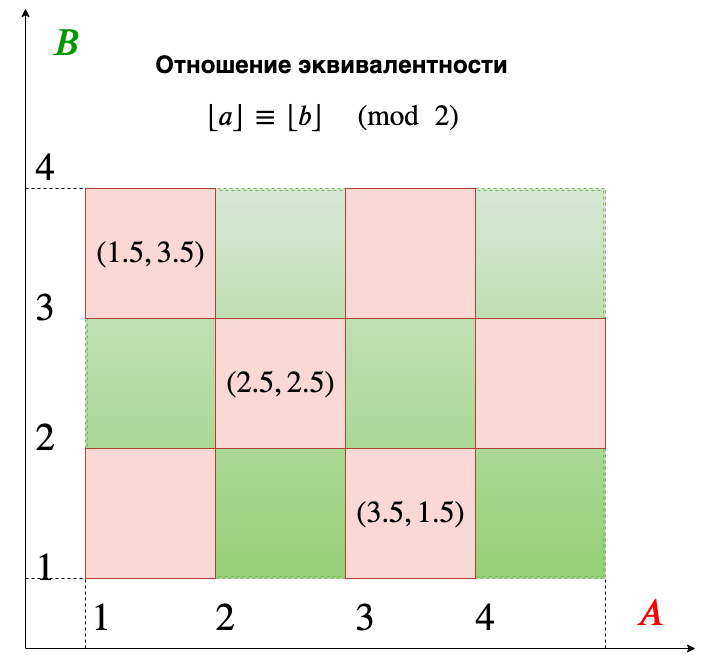
\includegraphics[scale=0.25]{../equiv.png}
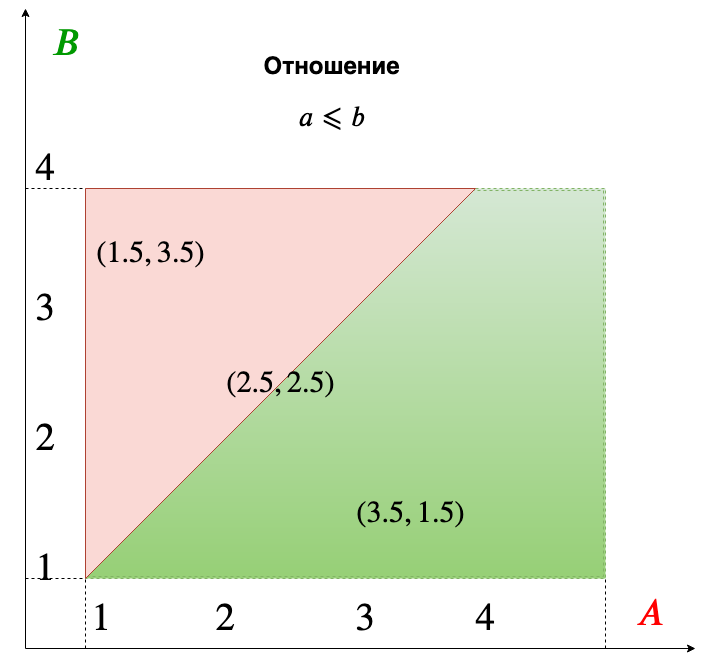
\includegraphics[scale=0.25]{../lessthan.png}
\end{center}


\item Докажите, что отношение сравнимости по любому заданному модулю является отношением эквивалентности на множестве целых чисел. Что представляют собой классы эквивалентности в этом случае?

\item Постройте фактормножество множества $\Z_9=\{0,1,2,3,4,5,6,7,8\}$ по отношению сравнимости по модулю $3$.

\item Что представляет собой фактор-множество произвольного множества $X$ по отношению равенства? Рассмотрите также случай $X=\emptyset$.

\item Докажите что два класса эквивалентности либо не перескаются, либо совпадают. Что можно сказать о сумме мощностей классов эквивалентности конечного множества?

\item \textit{Разбиением множества} $A$ называется такое множество непустых множеств $\{A_n\}$, что $A_i\cap A_j=\emptyset$ для всех $i,j$ ($i\ne j$) и, кроме того $A$ есть объединение всех $A_n$. Докажите, что
\ipunkt фактор-множество является разбиением; \ipunkt всякому разбиению соответствует единственное отношение эквивалентности, фактор-множество по которому совпадает с данным разбиением.

\item Числом Бэлла $B_n$ для натурального $n$ называется количество всех разбиений множества, состоящего из $n$ элементов. Найдите $B_5$ и $B_7$.


\end{enumerate}



\begin{comment}
\chapter{26. Функции и равномощность}
\end{comment}
\newchapter{Функции и равномощность}


\vrezka{Конспект: Глава 10, раздел 10.1 Теория множеств: отношения и функции, Глава 15, раздел 15.1 Мощности множеств.}

\subsection*{Справочные сведения}

Отношение $R\subseteq A\times B$ называется \ipunkt \textit{однозначным}, если из $(aRb\land aRc)$ следует $b=c$,
\ipunkt \textit{всюду определенным}, если $\forall a\in A\;\exists b\in B\; (aRb)$, \ipunkt \textit{всюду значным}, если $\forall b\in B\;\exists a\in A\;(aRb)$, \textit{обратно однозначным}, если из $(aRb\land cRb)$ следует $a=c$.

\textit{Функция} $f:A\to B$ --- это всюду определенное однозначное отношение $f$ между $A$ и $B$. Иначе говоря, функция $f$ каждому элементу из $A$ ставит в соответствие единственный элемент из $B$. Функция называется \ipunkt \textit{инъекцией}, если она является также обратно однозначным отношением, \ipunkt \textit{сюръекцией} --- если она является также всюду значным отношением, \ipunkt \textit{биекцией} --- если она сюръекция и инъекция одновременно.

Если $f:A\to B$ и $(a,b)\in f$, то пишут $b=f(a)$.

Множества $A$ и $B$ \textit{равномощны}, если между ними существует биекция. Равномощность множеств $A$ и $B$ записывается так: $|A|=|B|$.

Отношение $R^{-1} = \{(b,a)\mid (a,b)\in R\}$ называется \textit{обратным} к отношению $R$. Если $f$ --- сюръекция из $A$ в $B$ и отношение $f^{-1}$ является функцией из $B$ в $A$, то $f^{-1}$ называется \textit{обратной функцией} к функции $f$.

Пусть задано отношение $R\subseteq A\times B$. И пусть $X\subseteq A$, $Y\subseteq B$. Образом множества $X$ по отношению $R$ называется множество $R[X]=\{b\mid aRb\land a\in X\}$. Прообразом множества $Y$ по отношению $R$ называется множество $R^{-1}[Y]=\{a\mid aRb\land b\in Y\}$.

\textbf{Внимание!} При записи образа и прообаза множества мы используем \textit{квадратные скобки}, не следует путать их с круглыми, включающими аргумент функции.

Множество называется \textit{конечным}, если оно равномощно множеству $\{1, 2, \dots , n\}$ для
некоторого натурального $n$ или пусто. Говорят, что множество \textit{бесконечно}, если оно не является
конечным.

Множество называется \textit{счётным}, если оно равномощно множеству натуральных чисел $\N$.
 Говорят, что множество не более чем счётно, если оно конечно или счётно. Множество называется
 \textit{ несчётным}, если оно бесконечно и не является счётным.


\subsection*{Задачи}

\begin{enumerate}

\item Рассмотрим соответствие множества людей и множества всех возрастов (целых лет). В каком направлении соответствие между ними является функцией?
\item Рассмотрим соответствие множества людей и банковских счетов. Является ли это соответствие функцией хоть в каком-то направлении?
\item Доказать, что функция $f(x)=3x-7$ биективно отображает $\R$ в $\R$.
\item Доказать, что функция $g(x)=x^2+3x-6$ действует инъективно при $x\in[-3/2,+\infty)$.

\item Доказать, что прообраз $Y$ --- это образ $Y$ для обратного отношения.

\item Пусть $R\subseteq A\times B$ и $X_1,X_2\subseteq A$, $Y_1,Y_2\subseteq B$. Проверьте, что

\noindent\ipunkt $R[X_1\cup X_2] = R[X_1]\cup R[X_2]$;

\noindent\ipunkt $R^{-1}[Y_1\cup Y_2] = R^{-1}[Y_1]\cup R^{-1}[Y_2]$;

\noindent\ipunkt $R[X_1\cap X_2]\subseteq R[X_1]\cap R[X_2]$;

\noindent\ipunkt $R^{-1}[Y_1\cap Y_2]\subseteq R^{-1}[Y_1]\cap R^{-1}[Y_2]$.

Что изменится, если $R$ будет функцией? инъекцией? биекцией?

\item Привести примеры, когда $f[X_1\cap X_2]\ne f[X_1]\cap f[X_2]$, если $f:A\to B$.

\item Что можно сказать \ipunkt о равенстве множеств $X$ и $f^{-1}[f[X]]$; \ipunkt о равенстве множеств $Y$ и $f[f^{-1}[Y]]$, если такие множества определены?

\item Докажите, что равномощность является отношением эквивалентности, то есть
\ipunkt $|A| = |A|$;
\ipunkt если $|A| = |B|$, то $|B| = |A|$;
\ipunkt если $|A| = |B|$ и $|B| = |C|$, то $|A| = |C|$.

\item Докажите, что для любых множеств $X$ и $Y$ выполнено $|X \times Y | = |Y \times X|$.

\item Верно ли, что если $|A| = |B|$ и $|C| = |D|$, то
\ipunkt $|A \times C| = |B \times D|$;
\ipunkt $|A \cup C| = |B \cup D|$;
\ipunkt $|A \cap C| = |B \cap D|$?

\item Докажите, что следующие множества являются счётными:
\ipunkt множество чётных натуральных чисел;
\ipunkt множество нечётных натуральных чисел;
\ipunkt множество натуральных чисел без числа 2015;
\ipunkt множество целых чисел $\Z$.

\item Докажите, что всякое подмножество счётного множества не более чем счётно.

\item Докажите, что если $X$ счётно, а $Y$ конечно и непусто, то $X \times Y$ счётно.

\item Докажите, что следующие множества являются счётными:
\ipunkt объединение конечного числа счётных множеств;
\ipunkt прямое произведение двух счётных множеств;
\ipunkt объединение счётного числа различных конечных множеств;
\ipunkt объединение счётного числа счётных множеств.

\item Докажите, что множество рациональных чисел $\Q$ является счётным.

\item *Верно ли, что следующие множества являются счётными:
\ipunkt множество всевозможных конечных последовательностей нулей и единиц;
\ipunkt множество всевозможных русских «слов»;
\ipunkt множество конечных подмножеств множества $\N$?
\end{enumerate}




\begin{comment}
\chapter{27. Группы: основы}
\end{comment}
\newchapter{Группы: основы}

\vrezka{Конспект: Глава 2, раздел 2.1 Сдвиг, композиция сдвигов, группа, Глава 10, раздел 10.3 Пара слов о конечных группах.}

\subsection*{Справочные сведения}

Пара $(G,\circ)$, где функция $\circ:G\times G\to G$, называется \textit{группой}, если
\begin{enumerate}[{\color{darkred}G1}]
\item $(a\circ b)\circ c = a\circ (b\circ c)$ для любых $a,b,c\in G$ (ассоциативность);
\item существует элемент $\e\in G$ такой, что $a\circ \e=\e\circ a=a$ для любого $a\in G$ (единица);
\item для всякого $a\in G$ существует элемент $a^{-1}\in G$ такой, что $a\circ a^{-1}=a^{-1}\circ a=\e$ (обратный элемент).
\end{enumerate}

Группа называется \textit{абелевой} (\textit{коммутативной}), если групповая операция коммутативна, т.е. $a\circ b=b\circ a$ для всех $a,b\in G$.

Обозначение групповой операции по умолчанию будем пропускать, записывая $a\circ b$ как $ab$.

$H$ --- \textit{подгруппа} группы $G$, если $H\subseteq G$, $H$ замкнуто относительно групповой операции группы $G$ и групповая операция группы $G$ является групповой операцией в $H$. Множество $gH=\{gh\mid h\in H\}$ называется \textit{левым классом смежности} подгруппы $H$, множество $Hg=\{hg\mid h\in H\}$ --- \textit{правым классом смежности}.

\textit{Порядок группы} --- это количество ее элементов.

\textit{Индексом подгруппы} $H$ в группе $G$ называется количество различных смежных классов. Обозначение: $|G:H|$.

\subsection*{Задачи}


\begin{enumerate}
\item Показать, что единица и обратный элемент в группе определяются однозначно.

\item Ассоциативна ли операция $\circ$ на множестве $M$, если 
\ipunkt $M = \N$, $x\circ y = x^y$;
\ipunkt $M = \Z$, $x\circ y = x^2 + y^2$;
\ipunkt $M = \R$, $x\circ y = \sin x \cdot \sin y$?

\item Пусть на множестве $X$ задана операция $x\circ y$ и для нее выполняются тождества: $\forall x,y\in X\;$ $(x\circ y)\circ y=x$ и $y\circ(y\circ x)=x$. Доказать, что данная операция коммутативна, т.е. $x\circ y=y\circ x$.

\item Пусть на $\Z$ задана операция $n\circ m = n+m+nm=(1+n)(1+m)-1$. Каким аксиомам группы она удовлетворяет? Существует ли единица этой операции и как она выглядит? Существуют ли обратные элементы и для каких элементов?

\item Пусть $G$ --- группа и непустое множество $H\subseteq G$. Доказать, что если множество $H$ замкнуто относительно групповой операции и конечно, то оно является подгруппой группы $G$.

\item Доказать, что множество всех биекций на множестве $X$ образует группу с операцией композиции функций: $(f\circ g)(x)=f(g(x))$.

\item Доказать, что пересечение произвольного множества подгрупп группы $G$ является подгруппой группы $G$.

\item Доказать, что в произвольной группе правый и левый смежные классы подгруппы равномощны этой подгруппе.

\item Вывести из предыдущего утверждения \textbf{теорему Лагранжа}: порядок подгруппы делит порядок группы. Предполагается, что группа --- конечная.

\item Какое отношение эквивалентности соответствует разбиению группы $G$ на \ipunkt правые; \ipunkt левые классы смежности?

\item Доказать, что $m\Z$ является подгруппой в $\Z$ с операцией сложения. Найти все смежные классы этой подгруппы. Найти индекс подгруппы $m\Z$ в группе $\Z$, т.е. вычислить $|\Z:m\Z|$.

\item Доказать, что $\Q$ не содержит собственных подгрупп конечного индекса.

\item Доказать следующее обобщение теоремы Лагранжа. Пусть $A,B$ --- подгруппы группы $G$, и $A\subseteq B$. Индексы $|G:B|$ и $|B:A|$ конечны тогда и только тогда, когда $|G:A|$ конечен и $|G:A|=|G:B|\cdot|B:A|$.

\item Проверить, что $\{\id,(12)(34),(13)(24),(14)(23)\}$ является подгруппой группы $\Sb_4$ перестановок на 4 символах. Каков ее индекс в $\Sb_4$? Найдите ее правые и левые смежные классы в группе $\Sb_4$.

\item В группе $\Z_8^*$ найти обратные элементы: $3^{-1}, 5^{-1}, 7^{-1}$.

\end{enumerate}







\begin{comment}
\chapter{28. Циклические группы}
\end{comment}
\newchapter{Циклические группы}

\vrezka{Конспект: Глава 2, раздел 2.1 Сдвиг, композиция сдвигов, группа; Глава 10, раздел 10.3 Пара слов о конечных группах.}

\subsection*{Справочные сведения}

Традиционные обозначения и термины. Если групповая операция обозначается как '+', то группа называется \textit{аддитивной}, при этом нейтральный элемент обозначается за 0, а обратный элемент к элементу $g$ называется \textit{потивоположным} и записывается как $-g$. Обычно абелевы группы считаются аддитивными. Если групповая операция обозначается как '$\cdot$', то группа называется \textit{мультипликативной}, а знак операции, как правило, пропускается в записи формул, при этом нейтральный элемент обозначается за 1, а обратный элемент к элементу $g$ записывается как $g^{-1}$. Если группа состоит из отображений, а групповой операцией является композиция отображений, то нейтральный элемент обозначается $\id$, в остальном нотация соответствует мультипликативному варианту.


Кратную групповую операцию будем записывать с помощью натуральных чисел:
$$
ng = \underbrace{g+\dots+g}_{n\mbox{ раз}},\quad g^n = \underbrace{g\cdot\dots\cdot g}_{n\mbox{ раз}},
$$
где $n\in\N$, причем $0g=0$ и $g^0=1$ (в общем случае $g^0=\e$, где $\e$ --- нейтральный элемент). Для отрицательных коэффициентов полагаем:
$$
(-n)g = -(ng),\quad g^{-n} = (g^{-1})^n,
$$
где $n\in\N$.

Группа $G$ \textit{порождается} множеством $S\subseteq G$, если всякий элемент $g\in G$ можно представить в виде
$$
g = s_1^{\de_1}s_2^{\de_2}\dots s_n^{\de_n},
$$
где $s_k\in S$, $\de_k\in\Z$. В случае аддитивной группы данное представление принимает вид
$g = \de_1s_1+\de_2s_2+\dots+\de_ns_n$.

Обозначение: $G=\langle S\rangle$ --- множество $S$ порождает группу $G$. Если $S$ состоит из одного элемента $s$ (т.е. $G$ порождается степенями одного своего элемента), то пишут $G=\langle s\rangle$, при этом группа называется \textit{циклической}.

\textit{Порядок элемента} группы --- это его минимальная положительная степень, в которой данный элемент равен $\e$. Если такой степени не существует, то данный элемент имеет бесконечный порядок.



\subsection*{Задачи}

\begin{enumerate}
\item Доказать свойства степеней в группе:
$$
g^mg^n=g^{m+n},\quad (g^m)^n = g^{mn}
$$
(соответственно, $mg+ng=(m+n)g$ и $n(mg)=(nm)g$).

\item Доказать. что если $G$ --- конечная группа, то $g^n = g^{n\mod m}$, где $m$ --- порядок элемента $g$ в группе $G$.

\item Доказать, что если группа $G=\langle S\rangle$ конечная, то любой элемент $g\in G$ имеет представление $s_1^{m_1}\dots s_n^{m_n}$ для некоторых $s_k\in S$, где все $m_k$ --- неотрицательные целые числа.

\item Доказать, что в конечной группе порядок всякого элемента делит порядок группы.

\item Доказать, что группа $G$ четного порядка $|G|=2n$ обязательно содержит элемент $g\ne\e$ порядка 2. \textsl{Указание: представить $G$ как объединение пар $g,g^{-1}$}.

\item Является ли циклической группа \ipunkt $(\Z,+)$; \ipunkt $(\Z,\cdot)$?

\item Найдите порядок элемента $R_\ph$ в группе вращений окружности, если \ipunkt $\ph=\pi$; \ipunkt $\ph=\pi/3$; \ipunkt $\ph=\pi/6$; \ipunkt $\ph=32\pi/63$; \ipunkt $\ph=\pi\sqrt 2$; \ipunkt $\ph=0$.

\item Существует ли конечное множество образующих у следующих групп: \ipunkt группа движений прямой; \ipunkt группа движений окружности; \ipunkt группа движений правильного многогранника;

\item Доказать, что перестановочные элементы $g,h$ произвольной группы $G$, имеющие взаимно простые порядки $m,n$, порождают в $G$ циклическую подгруппу $H$ порядка $mn$, где $H=\langle g,h\rangle=\langle gh\rangle$. \textsl{Указание: использовать равенство $\gcd(m,n)=km+ln$.}

\item Показать, что $\Sb_n = \langle (12),(13),\dots,(1n)\rangle$.
\item Показать, что $\Sb_n = \langle (12),(123\dots n)\rangle$.
\item Показать, что знакопеременная группа $A_n$, $n\ge 3$, порождается циклами длины 3, причем
$$
A_n = \langle (1\,2\,3), (1\,2\,4), \dots, (1\,2\,n) \rangle.
$$

\item Показать, что порядок перестановки $\si\in\Sb_n$ (порядок циклической группы $\langle\si\rangle$) равен НОК длин независимых циклов, входящих в разложение $\si$.

\item Какую систему образующих можно предложить для мультипликативной группы $(\Q^+,\cdot)$ положительных рациональных чисел? \textsl{Указание: использовать ОТА}.

\item Показать, что все группы порядка 4 абелевы. \textsl{Указание: если для всех $x\in G$ имеем $x^2=\e$, то $abab=\e$ и, следовательно, $ab=ba$}.

\end{enumerate}




\begin{comment}
\chapter{29. Нормальные подгруппы. Гомоморфизмы}
\end{comment}
\newchapter{Нормальные подгруппы. Гомоморфизмы}

\vrezka{Конспект: Глава 2, раздел 2.1 Сдвиг, композиция сдвигов, группа; Глава 10, раздел 10.3 Пара слов о конечных группах.}

\subsection*{Справочные сведения}

Подгруппа $H$ группы $G$ называется \textit{нормальной}, если ее правые и левые смежные классы совпадают, т.е. $gH=Hg$ при любом $g\in G$. Обозначение: $H\triangleleft G$. Группа $G$ называется \textit{простой}, если она не имеет нетривиальных (отличных от $\{\e\}$ и $G$) нормальных подгрупп.

Множество классов смежности по нормальной подгруппе $H$ с операцией умножения $(g_1H)(g_2H)=(g_1g_2)H$ образует группу, которая называется \textit{факторгруппой} группы $G$ по нормальной подгруппе $H$ и обозначается $G/H$. Единицей факторгруппы является подгруппа $H$.

\textit{Гомоморфизмом} группы $G$ в группу $G'$ называется всякая функция $f:G\to G'$, сохраняющая групповую операцию, т.е. $f(ab)=f(a)f(b)$ для всех $a,b\in G$. \textit{Ядро гомоморфизма} --- это прообраз единицы: $\ker f=\{x\mid f(x)=\e'\}$, где $\e'$ --- нейтральный элемент группы $G'$.

Ядро гомоморфизма $f:G\to G'$ является нормальной подгруппой в группе $G$. Обратно: каждой нормальной подгруппе $H\triangleleft G$ соответствует гомоморфизм $f(a)=aH$, действующий из $G$ в $G/H$, для которого $\ker f=H$.

$f:G\to G'$ называется \textit{изоморфизмом} групп $G$ и $G'$, если $f$ --- гомоморфизм и биекция.



\subsection*{Задачи}

\begin{enumerate}
\item Найти факторгруппы: \ipunkt $\Z/n\Z$; \ipunkt $4\Z/12\Z$.
\item Доказать, что $\ker f\triangleleft G$, если $f:G\to G'$ --- гомоморфизм.

\item Доказать, что любая подгруппа абелевой группы нормальна.
\item Доказать, что $A_n\triangleleft \Sb_n$.

\item Доказать, что $\Z/p\Z$ --- простая группа, если $p$ --- простое число.

\item Доказать, что если $|G:H|=2$, то $H\triangleleft G$.

\item Доказать, что в группе $\Q/\Z$: \ipunkt каждый элемент имеет конечный порядок; \ipunkt для каждого натурального $n$ имеется в точности одна подгруппа порядка $n$.

\item Пусть $H\triangleleft G$ и $f:G\to G/H$ --- естественный гомоморфизм, т.е. $f(g)=gH$. Доказать, что $f$ --- гомоморфизм, \textit{эпиморфизм} (т.е. сюръективный гомоморфизм), а также, что $\ker f=H$.

\item Найти все нетривиальные подгруппы $\Sb_3$ Какие из них являются нормальными? Каким группам $\Z_m$ изоморфны факторы по данным нормальным подгруппам?

\item Показать, что \textit{группа Клейна} $V_4=\{\id,(12)(34), (13)(24), (14)(23)\}$ является нормальной в $\Sb_4$.

\item Рассмотрим на прямой точки $X,A,B,C,D$, предполагая, что все они попарно различны. Обозначим за $a$ разность точек $A-X$, которая равна длине отрезка $XA$, взятой со знаком направления (если $A$ справа от $X$, то с плюсом, иначе --- с минусом), а также $b=B-X$, $c=C-X$, $d=D-X$. Запишем \textit{двойное отношение}
$$
\la = [A;B;C;D] = \frac{(c-a)(d-b)}{(c-b)(d-a)}.
$$

Докажите, что двойное отношение не зависит от выбора точки $X$.

\item Пусть точки $A,B,C,D$ пронумерованы цифрами $1,2,3,4$. Через $\la(\si)$ обозначим двойное отношение $[\si(A);\si(B);\si(C);\si(D)]$, где $\si\in\Sb_4$, т.е. является перестановкой на 4 символах. Покажите, что
$$
\la(\si) \in \Lambda = \left\{\la,\frac{1}{\la},1-\la,\frac{1}{1-\la},1-\frac{1}{\la},\frac{\la}{1-\la}\right\}
$$
при любом $\si$.

\item Показать, что если на множестве $\Lambda$ ввести операцию композиции (т.е. рассматривать его элементы как функции от аргумента $\la$ и подставлять одну в другую), то получится группа, изоморфная $\Sb_3$. Что в этой группе является единицей?

\item Покажите, что перестановки $\Sb_4$, сохраняющие двойное отношение, --- это перестановки группы Клейна $V_4$.

\item Какой группе изоморфна группа $\Sb_4/V_4$? Как это связать со свойствами двойного отношения? Какой эпиморфизм $\Sb_4\to\Sb_3$ можно задать с помощью двойного отношения?

\item Рассмотрим группу движений правильного $n$-угольника. Два движения будем называть эквивалентными, если их композиция является поворотом (или $\id$). Докажите, что это и в самом деле отношение эквивалентности, постройте классы эквивалентности, постройте факторгруппу на этих классах. Какова ее таблица умножения?

\end{enumerate}









\begin{comment}
\chapter{30. Сопряжение}
\end{comment}
\newchapter{Сопряжение}

\vrezka{Конспект: Глава 10, раздел 10.3 Пара слов о конечных группах.}

\subsection*{Справочные сведения}

Для группы $G$ и двух ее элементов $x,g\in G$ элемент $x^{-1}gx$ называется \textit{сопряженным} $g$ \textit{при помощи} $x$ и обозначается $g^x$. При этом элементы $g$ и $h$ называются \textit{сопряженными}, если при некотором $x$ имеет место равенство $g^x=h$. Пишем: $g\sim h$.

Классом сопряженности элемента $g$ называется множество $g^G=\{g^x\mid x\in G\}$.

Критерий нормальной подгруппы. Пусть $H$ --- подгруппа группы $G$, тогда $H\triangleleft G$ тогда и только тогда, когда $H$ есть объединение некоторых классов сопряженности. Отсюда, в частности, следует, что нормальные подгруппы следует искать только среди объединений классов сопряженности (в конечной группе: если такое объединение замкнуто относительно групповой операции, то оно является нормальной подгруппой).


\subsection*{Задачи}

\begin{enumerate}
\item Доказать свойства сопряжения: \ipunkt $g^{xy}=(g^x)^y$; \ipunkt $(gh)^{x}=g^xh^x$; \ipunkt $(g^{-1})^x=(g^x)^{-1}$;\label{sopr}

\item Доказать, что отношение сопряженности элементов является отношением эквивалентности и классы сопряженности либо не пересекаются либо совпадают.

\item Доказать, что $g^x$, как функция от $g$, является автоморфизмом $G$ при любом $x$.\label{autG}

\item Доказать, что если $f:G\to G'$ гомоморфизм и $g\in\ker f$ и $g\sim h$, то $h\in\ker f$.

\item Опишите перестановки, сопряженные пеерестановке $(13)(24)$ в группе $\Sb_4$.

\item Доказать, что при сопряжении при помощи \ipunkt перестановки $(12)$; \ipunkt любой транспозиции; \ipunkt любой перестановки цикловая структура перестановки (т.е. количество циклов определенной длины) не меняется. \ipunkt Обратно: если перестановки имеют одинаковую цикловую структуру, то они сопряжены.

\item Опишите классы сопряженности в группе \ipunkt $\Sb_3$; \ipunkt $\Sb_4$

\item Пусть $\si\in\Sb_n$. И пусть $\tilde{\si}(\tau)=\tau^\si=\si^{-1}\tau\si$. Из задачи \ref{autG} следует, что 
$\tilde{\si}$ --- автоморфизм $\Sb_n$, т.е. биекция, т.е. $\tilde{\si}\in \Sb(\Sb_n)$.
\begin{enumerate}[a)]
\item Что представляет собой автоморфизм $\tilde{\id}$?
\item Занумеруем элементы $\Sb_3$ числами от 1 до 6 в каком-либо порядке. Тогда автоморфизм $\tilde{\si}$ можно записать как элемент $\ph(\si)\in\Sb_6$. Какая перестановка $\ph(\si)$ из $\Sb_6$ соответствует \ipunkt $\si=(12)$; \ipunkt $\si=(13)$; \ipunkt $\si=(123)$?
\item Доказать, что $\tilde{\si}(\al\circ\be)=\tilde{\si}(\al)\tilde{\si}(\be)$. Сравнить с \ref{sopr}.
\item Доказать, что соответствие $\si\mapsto\ph(\si)$, определенное выше и действующее из $\Sb_n$ в $\Sb_{n!}$, является гомоморфизмом при любом выборе нумерации элементов $\Sb_n$.
\end{enumerate}

\item Гомоморфизм $\ph(\si):\Sb_n\to\Sb_{n!}$, определенный в предыдущей задаче, можно рассматривать не на всем $\Sb_n$, а только на перестановках, в ходящих в один класс сопряженности $K$. Доказать, что сужение $\ph|_K$ является гомоморфизмом из $\Sb_n$ в $\Sb_{|K|}$, где $|K|$ --- мощность множества $K$.

\item Пусть $K=(12)^{\Sb_3}$. Доказать, что $\ph|_K:\Sb_3\to\Sb_3$ --- изоморфизм.\label{(12)}

\item Пусть $K=(123)^{\Sb_3}$. Доказать, что $\ph|_K:\Sb_3\to\Sb_2$ --- отображение знака, т.е. четным перестановкам сопоставляется $\id$, а нечетным --- транспозиция. \label{(123)}

\item Найти ядра гомоморфизмов из задач \ref{(12)} и \ref{(123)}.

\item Найти ядро гомоморфизма $\ph|_K:\Sb_4\to\Sb_{24}$, если $K=((12)(34))^{\Sb_4}$.

\item Доказать, что если $f:\Sb_n\to\Sb_m$ --- гомоморфизм и $(12)\in\ker f$, то $\ker f=\Sb_n$.
\end{enumerate}





\begin{comment}
\chapter{31. Движения плоскости: определения}
\end{comment}
\newchapter[определения]{Движения плоскости:}

\vrezka{Конспект: Глава 11, раздел 11.1 Виды движений плоскости. Теорема Шаля.}

\subsection*{Справочные сведения}

Движение плоскости --- это всякое отображение $x\mapsto f(x)$, которое точкам плоскости ставит в соответствие точки плоскости, причем с сохранением расстояния, т.е. $|AB|=|f(A)f(B)|$ (отрезок $AB$ переходит в равный ему по длине отрезок $f(A)f(B)$).

Виды движений плоскости:
\begin{enumerate}[\color{darkred}P1]
\item $T_v$: параллельный перенос на вектор $v$;
\item $R_\al^O$: поворот с центром $O$ на угол $\al$;
\item $S_l$: отражение относительно прямой $l$ (частный случай $T_vS_l$ при $v=0$);
\item $T_vS_l$: скользящая симметрия со сдвигом на вектор $v$ и симметрий относительно прямой $l\parallel v$.
\end{enumerate}




\subsection*{Задачи}






%Глава 8

%\item Проверить, что $\Z_m$ удовлетворяет аксиомам кольца.

